\documentclass[11pt, a4paper, german]{article}
\usepackage[utf8]{inputenc}
\usepackage[ngerman]{babel}
\usepackage{amsmath}
\usepackage{amsthm}
\usepackage{amsfonts}
\usepackage{amssymb}
\usepackage{color}
%\usepackage{algorithmicx}
%\usepackage[compatible]{algpseudocode}
\usepackage{algorithm}
%\usepackage{algorithmic}
\usepackage{algpseudocode}
\usepackage{makeidx}
\usepackage{graphicx}
\usepackage{tabularx}
\usepackage{bbm}
\usepackage{BA_Titelseite}
\usepackage{bm}
\usepackage[colorlinks=true, pdfborder={0 0 0}, linkcolor=blue, citecolor=magenta]{hyperref}
\bibliographystyle{unsrt}



%Namen des Verfassers der Arbeit
\authornew{Boris Prochnau}

%Geburtsdatum des Verfassers
\geburtsdatum{22. Dezember 1989}
%Gebortsort des Verfassers
\geburtsort{Tartu}
%Datum der Abgabe der Arbeit
\date{\today}

%Name des Betreuers
% z.B.: Prof. Dr. Peter Koepke
\betreuer{Betreuer: Prof. Dr. Anton Bovier,\\ Dipl. Martina Baar und Dr. Loren Coquille}
%Name des Instituts an dem der Betreuer der Arbeit tätig ist.
%z.B.: Mathematisches Institut
\institut{Institut für Angewandte Mathematik}
%Titel der Bachelorarbeit
\title{Simulation einer stochastischen Populationsdynamik}
%Do not change!
\ausarbeitungstyp{Bachelorarbeit Mathematik}

\theoremstyle{plain}
\newtheorem{satz}{Satz}[section]
\newcommand{\eps}{\ensuremath{\varepsilon}}
\newcommand{\tvec}[2]{\begin{pmatrix}#1\\#2\end{pmatrix}}
\newcommand{\trvec}[3]{\begin{pmatrix}#1\\#2\\#3\end{pmatrix}}


\begin{document}


\maketitle
\setcounter{tocdepth}{2}
\tableofcontents


\clearpage
\section{Einleitung}
Diese Bachelorarbeit behandelt die Entwicklung eines Programms zur Simulation einer Populationsdynamik. Dazu wird erst ein Grundlegendes Modell vorgestellt, welches den zu simulierenden BPDL-Prozess beschreibt.\\
Das Programm sollte jedoch nicht nur in der Lage sein diesen Prozess zu simulieren, sondern auch die Approximation von Grenzwertprozessen, die aus dem BPDL-Prozess gewonnen werden. Dazu z"ahlt auch der sogenannte "{}TSS-Prozess"{}. Die Simulation einer Approximation des "{}TSS-Prozesses"{} ist besonders interessant und wird im Kapitel 3 eingef"uhrt und sp"ater im Kapitel 7 genauer beschrieben.\\
Alle Simulationen sollen auf dem selben Modell basieren.\\
Jedes Lebewesen einer Population (z.B. Pflanzen, Zelle oder Tier) wird durch ein Merkmal beschrieben. Diese Merkmale erzeugen Dynamik in der Population, indem sie z.B. Gr"o"se, Essensaufnahme, Fortpflanzungsrate oder Konkurrenz zu anderen Merkmalen angeben.\\
In unserem Modell besteht ein Merkmal aus einer asexuellen Fortpflanzungsrate und zwei Todesraten. Die Todesraten bestehen aus einer nat"urlichen Todesrate und einer Todesrate, die durch Wettbewerb zu jedem anderen Lebewesen entsteht. Man bemerkt schon, dass ein Individuum in diesem Modell nur sterben, t"oten (durch Wettbewerb) oder sich fortpflanzen kann. Wobei das Interessante an der Dynamik ist, dass die wettbewerblichen Todesraten der Individuen von den Populationsgr"o"sen abh"angen und damit nicht trivial machen.\\
Desweiteren umfasst das Modell eine Mutationswahrscheinlichkeit. Diese Mutation bezieht sich nicht auf bereits in der Population lebende Wesen, sondern auf neugeborene Individuen.\\
Desweiteren werden wir viele Individuen auf wenigen Merkmalen verteilt simulieren, weshalb die Entwicklung der Population und nicht die der Individuen das Ziel der Simulation ist (im Gegensatz zu \cite{fournier2004microscopic}). Deshalb wird man im simulierten Prozess zwar Tode und Geburten in Merkmalen verfolgen k"onnen, aber nicht, welches Individuum dieses Ereignis ausl"ost. Der "Ubergang zu dieser Sichtweise wird n"aher im 2. Kapitel beschrieben.\\
Haupts"achlich wird in dieser Arbeit beschrieben, wie sich dieses Modell und seine Eigenschaften auftrennen oder zusammenfassen lassen um m"oglichst effizient und sicher ein Programm zur Simulation eines entsprechenden Prozesses zu implementieren. Dabei wird oft auf moderne Methoden zur"uck gegriffen, die eine m"oglichst unabh"angige Strukturierung der Schritte w"ahrend eines Ablaufs voraussetzten.\\
Schlie"slich wird auch beschrieben, was eine Simulation leisten kann, sollte und was diese Simulation tats"achlich tut. Z.B. sollte die graphische Darstellung des Prozesses die M"oglichkeit bieten, beobachten zu k"onnen, ob sich ein Merkmal unter anderen durchsetzten kann, es einen stabilen Zustand annimmt oder sich dem Tod entgegen strebt.


\clearpage
\section{Modell}
Das verwendete Model wurde in \cite{Bolker_Spatial_moment,Bolker1997179,raey_Dieckmann_Law} eingef"uhrt. Bei asexueller Vermehrung nutzt das Modell die drei grundlegenden Mechanismen von Darwins Evolutionslehre: Vererbung, Variation (Mutationen) und Selektion durch Wettbewerb um eine Menge von Merkmalen f"ur Individuen zu beschreiben. Diese bestimmen die F"ahigkeit des Individuums zu "uberleben und sich fortzupflanzen. Der daraus resultierende zeitstetige Sprung-Prozess wird BPDL-Prozess (nach Bolker, Pacala, Dieckmann und Law) genannt.\\
Ziel wird es sein, zwei spezielle BPDL-Grenzwert-Prozesse simulieren zu k"onnen.
	\subsection{Grundlagen}
	Sei $ X $ der endliche diskrete Raum der Merkmale. Jedes Individuum hat genau ein solches Merkmal $ x \in X $ und ist vollst"andig durch dieses charakterisiert. Es ist hilfreich sich X als Indexmenge $ X = \{1,\dots, n\} $ vorzustellen, die abgez"ahlte Merkmale enth"alt. Das entspricht auch der Interpretation von X aus Sicht der Simulation. Der "Ubersicht halber werden Elemente aus $ X $ jedoch mit $ x,y \in X $ angesprochen. Ein allgemeineres Modell findet sich in \cite{raey}.\\
	F"ur jedes Individuum mit Merkmal $ x \in X $ gilt:
	\begin{itemize}
		\item Jedes Individuum kann sich nur asexuell fortpflanzen oder sterben.
		\item Fortpflanzungs- und Todeszeitpunkte k"onnen durch sogenannte exponentielle Uhren beschrieben werden (wie in \cite[S. 3]{fournier2004microscopic}). Diese Uhren haben exponentiell verteilte Weckzeiten. Durch die Gedächtnislosigkeit der Exponentialverteilung und wegen des Wettbewerbs, können und müssen alle Uhren nach dem ersten Klingeln neu gestellt werden. Durch den Einfluss des Wettbewerbs ist jede Todesrate abh"angig von der Anzahl an Konkurrenten, die durch das zuerst eintretende Ereignis beeinflusst wird. 
		\item Bei einer Fortpflanzung kann eine Mutation auftreten. D.h. die Fortpflanzung des Individuums mit Merkmal $ x \in X $ kann in der Geburt eines Individuums mit Merkmal $ y \in X $ resultieren. Die H"aufigkeit dieser Ereignisse wird durch die Mutationswahrscheinlichkeit beschrieben.
	\end{itemize}
	Sp"ater wird deutlich, dass die Zur"uckstellbarkeit der Uhren entscheidend ist, um die Sichtweise von der Ebene des Individuums auf die der gesamten Population zu heben.\\
	Diese Todes und Fortpflanzungs- Ereignisse eines Individuums haben feste Raten, die das dazugeh"orige Merkmal beschreiben.\\
	
	\begin{tabular}{r p{26em}}
		$ b(x) $: & Ist die Geburtenraten durch ein Individuum mit Merkmal $ x $.\\
		$ d(x) $: & Ist die natürliche Todesrate. Im Folgenden wird stets vorausgesetzt, dass ein Merkmal "uberlebensf"ahig ist. Also $ b(x) - d(x) > 0 $.\\
		$ c(x, y) $: & Ist die Todesrate durch Wettbewerb, die ein Individuum $ y $ auf $ x $ aus"ubt. Diese Interpretation orientiert sich an \cite{raey}, w"ahrend u.a. in \cite{Champagnat20061127} ein symmetrischer Wettbewerbskern verwendet wird. Im Gegensatz zu vorher kann der Wettbewerb ein konkurrierendes Merkmal zum Aussterben zwingen.\\
		$ \mu $: & Ist die Mutationswahrscheinlichkeit "{}auf die Nachbarn"{} mit je $ \frac{\mu}{2} $ pro Nachbar. \\
	\end{tabular}\\

	Alle erw"ahnten Raten sind wie in \cite{fournier2004microscopic} endlich und positiv. \\
	Schlie"slich lassen sich durch Superpositionsprinzip der Exponentialverteilung die beiden Todesraten zu einer gemeinsamen Todesrate zusammenfassen oder die arteigene Geburtenrate beschreiben.\\
	
	\begin{tabular}{ r p{18em} }
		$ b(x) \cdot (1 - \mu) $ & Ist die arteigene Geburtenrate eines Individuums mit Merkmal $ x $, also mutationsfreie Geburten.\\
		$ d(x) + \sum_{i=1}^{N_t} c(x, x_i) $ & Ist die gesamte Todesrate eines Individuums mit Merkmal x (mit $ N_t \hat{=} $ \#Individuen zur Zeit t mit Merkmal $ x $ und $ x_i $ das Merkmal des i-ten Individuums).\\
		$ d(x) + \sum_{y \in X} c(x,y) \cdot n_t(y) $ & Ist auch die gesamte Todesrate, diesmal jedoch "uber die Merkmale summiert, mit $ n_t(x) \hat{=} \text{\#Individuen}$ zur Zeit t mit Merkmal $ x $.
	\end{tabular}\\
	
	Im Unterschied zu \cite{Champagnat20061127} sind wir an der Entwicklung einer gro"sen Population mit wenigen Merkmalen interessiert. Deswegen ist es unpraktisch weiterhin die Raten jedes Individuums zu berechnen.\\
	Die letzte Darstellung der Todesrate ist z.B. praktischer f"ur die Betrachtung der Population durch den Fokus auf die Merkmale. "Ahnlich k"onnen weitere Ereignisse zusammengefasst werden, so dass man z.B. eine Todesrate und eine arteigene Geburtenrate der Merkmale erstellen kann:
	
	\begin{itemize}
		\item Die \textbf{Fortpflanzungsrate} des Merkmals $ x $: 
		\[ \tilde{B}(x) = b(x) \cdot n_t(x) \]
		Diese beschreibt die Rate mit der Fortpflanzungen innerhalb des Merkmals x stattfinden (nicht die Geburten innerhalb x!).\\
		\item Die arteigene Geburtenrate (\textbf{Wachstumsrate}) des Merkmals $ x $ ist von besonderem Interesse und ist das, womit wir folgend haupts"achlich arbeiten werden: 
		\begin{align*}
			B(x)  & = (1 - \mu) \cdot b(x) \cdot n_t(x)\\
				  & + \frac{\mu}{2} \cdot \underbrace{b(x+1) \cdot n_t(x+1)}_{\text{Mutation von rechts}} \cdot \mathbbm{1}_{x<n}\\
				  & + \frac{\mu}{2} \cdot \underbrace{b(x-1) \cdot n_t(x-1)}_{\text{Mutation von links}} \cdot \mathbbm{1}_{x>1}
		\end{align*}
		Hierbei ist zu beachten, dass: $ \sum_{x \in X} B(x)  = \sum_{x \in X} \tilde{B}(x)$, da die Mutationen von rechts und links per Teleskopsumme den Faktor $ (1-\mu) $ ausgleichen.
		
		\item Die \textbf{Todesrate} des Merkmals $ x $:
		\[ D(x) = \underbrace{n_t(x) \cdot d(x)}_{\text{intrinsische Todesrate}} + \underbrace{n_t(x) \cdot \sum_{y=1}^{n} c(x,y) \cdot n_t(y)}_{\text{wettbewerbliche Todesrate}}  \]
	\end{itemize}
	Das entspricht zwei wesentlichen exponentiellen Uhren pro Merkmal. Eine für Tod und eine für Geburt innerhalb des Merkmals.\\
	F"ur die Simulation ist eine Gesamtrate für das Eintreten eines Ereignisses praktischer. Auf diese Weise wird nur auf das Eintreffen einer Uhr gewartet.
	\begin{itemize}
		\item Ereignisrate des Merkmals $ x $ (Trait Rate):
		\[ TR(x) = B(x) + D(x) \]
		\item Totale Ereignis Rate (Total Event Rate): 
		\[ TER = \sum_{x \in X} TR(x)\]
	\end{itemize}
	Mit der Totalen Ereignisrate gibt es eine Rate, die es erlaubt eine Zufallsvariable für das Eintreffen einer Variable zu ziehen. Anschließend ist es nur noch erforderlich (mit der Ziehung zwei weiterer Zufallsvairablen) festzustellen, welchem Merkmal welches Ereignis zukommt. Das Zusammenfassen der Raten vereinfacht es dem Programm sp"atere Auswertungen und Funktionen bereitzustellen. So l"asst sich z.B. aus der Geburtenrate (Wachstumsrate) eines ausgestorbenen Merkmals die Mutationsrate ablesen, ohne weitere Berechnungen machen zu m"ussen.\\
	
	\subsection{BPDL-Prozess}
	Eine auf diesem Modell basierende Population wird durch folgendes Punktma"s beschrieben:
	\[ \nu_t = \sum_{i=1}^{N_t} \delta_{x_i}, \quad x_i \hat{=} \text{Das Merkmal des i-ten Individuums} \]
	Es bildet Merkmale auf die Anzahl ihrer Repr"asentanten ab.\\
	Mit Zeitpfaden ist $ \nu_t $ ein stochastischer Prozess, genauer ein Markov Sprung Prozess auf dem Ma"sraum:
	\[ \nu_t \in M(X) = \left\{ \sum_{i=1}^{m} \delta_{x_i}, m \in \mathbb{N}, x_1, \dots, x_n \in X \right\} \]
	Man erkennt leicht die Sprungeigenschaft:
	\[ \int_X 1 \text{ } \nu_t(dx) = N_t 
	\text{ und }
	\int_X \mathbbm{1}_y(x) \text{ } \nu_t(dx) = n_t(y) \]
	Normalerweise geh"ort zum Model des BPDL-Prozesses, dass die Mutationen auf einem beliebigen Merkmal (nicht nur den Nachbarn) landen k"onnen und der Raum der Merkmale nicht unbedingt diskret sein muss. Eine Mutationswahrscheinlichkeit h"angt in diesem Fall vom Merkmal ab, also $ \mu(x) $. Und der Mutant hat dann Merkmal $ x + h $, wobei h eine zentrierte Zufallsvariable mit Dichte $ m(x,dh) $ auf $ (X - x) $ ist.
	F"ur einen solchen Prozess w"are der Generator definiert als:
	\begin{align*}
		L(\phi(\nu)) &= \int_{X} b(x)(1-\mu)[\phi(\nu + \delta_x) - \phi(\nu)]\nu(dx)\\
					  &+ \int_{X}\int_{\mathbb{R}^d} b(x) \cdot \mu [\phi(\nu + \delta_{x+z}) - \phi(\nu)] m(x,dz) \nu(dx)\\
				  	  &+ \int_{X} d(x)[\phi(\nu - \delta_x) - \phi(\nu)]\nu(dx)\\
				 	  &+ \int_{X} \left( \int_{X} c(x,y) \nu(dy) \right) [\phi(\nu - \delta_x) - \phi(\nu)]\nu(dx)
	\end{align*}
	mit $ \phi: M \to \mathbb{R} $. \\
	Dieser beschreibt die erwartete "Anderung von $ \nu $ zur Zeit $ t $. Man erkennt, dass der Generator unabh"angig von $ t $ ist, da er nur mit Zeitunabh"angigen Parametern $ b, d, c, \mu $ konstruiert wurde. Nat"urlich ist der verwendete Prozess $ \nu_t $ abh"angig von t, weshalb man $ \frac{d}{dt}\mathbb{E}\phi(\nu_t) = L\phi(\nu_t) $ schreiben kann.\\
	Mit unserem diskreten Raum X und der konstanten Mutationswahrscheinlichkeit zu Nachbarn vereinfacht sich der Generator. Der f"ur unser Model angepasste Generator hat somit folgende Form:
	\begin{align}
	\begin{split}
		L(\phi(\nu)) &= \sum_{x \in X} b(x)(1-\mu)[\phi(\nu + \delta_{x}) - \phi(\nu)] \cdot n(x)\\
		&+ \sum_{y \sim x}b(x) \cdot \frac{\mu}{2} \cdot 
 [\phi(\nu + \delta_{y}) - \phi(\nu)] \cdot n(x)\\		 
		&+ \sum_{x \in X} \left(d(x) + \sum_{y \in X} c(x,y) \cdot n(y)\right)[\phi(\nu - \delta_{x}) - \phi(\nu)] \cdot n(x) \label{GeneratorDiskret}
	\end{split}
	\end{align}
	mit $ \phi: M \to \mathbb{R} $


\clearpage
\section{Eigenschaften des BPDL-Prozesses}
In diesem Kapitel werden Eigenschaften des Prozesses n"aher untersucht, die sp"ater oft bei der Simulation sichtbar sein sollen. Zun"achst wird dabei die Normalisierung eingef"uhrt, die es auch einfacher macht Aussagen "uber das erwartete Verhalten des Prozesses bzw. der Population zu machen. 

	\subsection{Normalisierung des BPDL-Prozesses}
	Wie schon zuvor erwähnt ist es für uns wichtig die Tode und Geburten nicht auf der Ebene des Individuums, sondern der gesamten Population zu betrachten. Dazu wird die LPA(Large Population Approximation) Normalisierung aus \cite{fournier2004microscopic} eingeführt.\\
	Hierfür wird der Prozess mit einem Parameter K skaliert und es ergibt sich eine neue Zufallsvariable:
	\[ \nu_t^K := \frac{1}{K} \nu_t \]
	Um f"ur $ \nu_t^K $ das selbe Verhalten wie f"ur $ \nu_t $ zu erhalten, m"ussen einige Anpassungen vorgenommen werden.\\
	Zun"achst wird die Anfangsgröße $ n_0^K $ der Population proportional zu K gewählt.
	Die Raten für Geburten und natürliche Tode der Individuen bleiben unverändert. Da die Populationsgröße jedoch quadratisch in die Wettbewerbsrate einfließt, sollte $ c_K(x,y) = \frac{c(x,y)}{K} $ gelten, da sonst die K-fach erh"ohte Population mit einem intensiven Aussterben den Vergleich verf"alschen w"urde. \\
	Ein Beispiel f"ur eine LPA-Normalisierung sieht folgendermaßen aus:
	\begin{figure}[H]
		\centering
		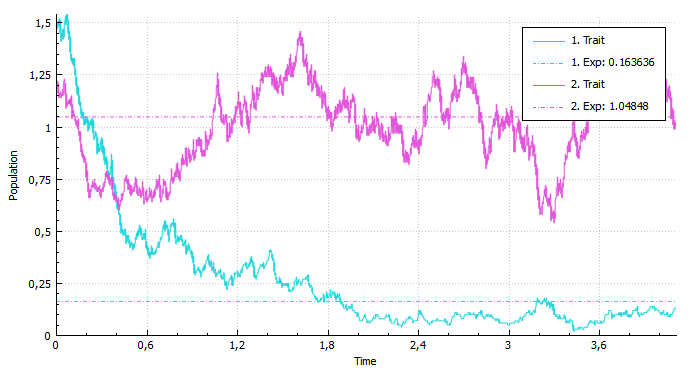
\includegraphics[width=1\linewidth]{./Pictures/LPANormalisierungK100}
		\caption[LPAK100]{LPA Normalisierung mit K=100}
		\label{LPA Normalisierung K=100}
	\end{figure}
	\begin{figure}[H]
		\centering
		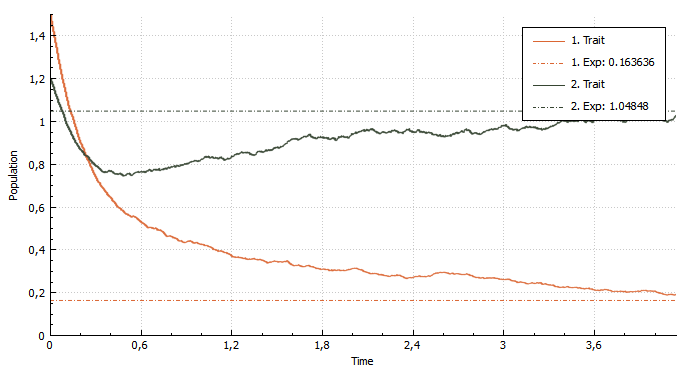
\includegraphics[width=1\linewidth]{./Pictures/LPANormalisierungK10000}
		\caption[LPAK100]{LPA Normalisierung mit K=10000}
		\label{LPA Normalisierung K=10000}
	\end{figure}
	Was in beiden Abbildungen jetzt schon auff"allt ist, dass die Population f"ur kleine K fast sofort aussterben w"urde, weil sich die Merkmale auf sehr geringen Populationen in ein Gleichgewicht einpendeln wollen.\\
	F"ur den Prozess $ \nu_t^K $ "andert sich der Generator ganz einfach zu:
	\begin{align*}
		L^K(\phi(\nu^K)) &= \int_{X} b(x)(1-\mu)\left[\phi\left(\nu^K + \frac{\delta_x}{K}\right) - \phi(\nu^K)\right]K\nu^K(dx)\\
			  &+ \int_{X}\int_{\mathbb{R}^d} b(x) \cdot \mu \left[\phi\left(\nu^K + \frac{\delta_{x+z}}{K}\right) - \phi(\nu)\right] m(x,dz) K \nu^K(dx)\\
		  	  &+ \int_{X} d(x)\left[\phi\left(\nu^K - \frac{\delta_x}{K}\right) - \phi(\nu^K)\right]K\nu^K(dx)\\
		 	  &+ \int_{X} \left( \int_{X} c_K(x,y) K \nu^K(dy) \right) \left[\phi(\nu^K - \frac{\delta_x}{K}) - \phi(\nu^K)\right]K\nu^K(dx)
	\end{align*}
	und in unserem Fall zu:
	\begin{align}
	\begin{split}
			L^K(\phi(\nu^K)) &= \sum_{x \in X} b(x)(1-\mu)\left[\phi\left(\nu^K + \frac{\delta_x}{K}\right) - \phi(\nu^K)\right]K \cdot n(x)\\
			&+ \sum_{y \sim x}b(x) \cdot \mu \cdot 
		 \left[\phi\left(\nu^K + \frac{\delta_y}{K}\right) - \phi(\nu^K)\right]K \cdot n(x)\\		 
			&+ \sum_{x \in X} \left(d(x) + \sum_{y \in X} c_K(x,y) K \cdot n(y)\right)\\
			&\cdot \left[\phi\left(\nu^K - \frac{\delta_x}{K}\right) - \phi(\nu^K)\right]K \cdot n(x) \label{GeneratorDiskretK}
	\end{split}
	\end{align}

	\subsection{LPA f"ur zwei Merkmale ohne Mutation}
	Falls mit $ K \to \infty $ auch $ n_0^K \to n_0 $ folgt, dann l"asst sich beweisen, dass das System gegen ein deterministisches System konvergiert $ \nu_t^K \xrightarrow{K} n_t $. Exemplarisch gehen wir von einem Fall von zwei Merkmalen ohne Mutation aus, jedoch l"asst es sich auf d Merkmale auch mit Mutation erweitern. Dieses Beispiel ist f"ur den TSS-Fall besonders interessant.\\
	Ein solches deterministisches System muss folgende Differentialgleichung erf"ullen:
	\begin{align}
	\begin{split}
		\dot{n}(x) &= n(x) \left( b(x) - d(x) - c(x,x) n(x) - c(x,y) n(y) \right), \quad n_0(x) = n_{0,x}\\
		\dot{n}(y) &= n(y) \left( b(y) - d(y) - c(y,y) n(y) - c(y,x) n(x) \right), \quad n_0(y) = n_{0,y} \label{Differentialgleichung}
	\end{split}
	\end{align}
	
	Um die Konvergenz zeigen zu k"onnen, verwenden wir ein Theorem aus \cite[Kapitel 11, Thm 2.1]{ethier2009markov}.\\
	Daf"ur wird zun"achst erl"autert, ob unser Modell die Bedingungen aus \cite{ethier2009markov} erf"ullt. Zu diesem Zweck wird unser mutationsfreies Modell in eine passende Notation aus \cite{ethier2009markov} "ubersetzt.\\
	Sei $ l \in \{ \binom{1}{0}, \binom{-1}{0}, \binom{0}{1}, \binom{0}{-1} \} $ und $ \beta_l : \mathbb{R}^2 \to \mathbb{R}_+ $. Mit $ l $ kann man das Merkmal und Ereignis auffassen, w"ahrend $ \beta_l $ eine Ratenfunktion ist, welche die Raten eines Merkmals und Ereignisse einer Population darstellt.\\
	Nat"urlich kann bei uns nur einem Merkmal ein Ereignis wiederfahren. Deswegen werden unsere $ l $ stets Einheitsvektoren sein, die auf das Merkmal verweisen mit Vorzeichen, die auf das Ereignis deuten.\\
	Z.B. $ l = \binom{0}{-1} $ meint einen Tod im zweiten Merkmal.\\
	Da $ \beta_l $ eine Population als Vektor erwartet, werden wir unsere Population mit $ n_t = \binom{n_t(x)}{n_t(y)} $ beschreiben. Daraus ergibt sich f"ur das $ \beta $ mit obigem Beispiel:
	\[ \beta_{\binom{0}{-1}}(n_t)  = \beta_{\binom{0}{-1}}\tvec{n_t(x)}{n_t(y)} = d(y) \cdot n(y) + \left(\sum_{x \in X} c(y,x)n(x)\right) \cdot n(y) \]
	dementsprechend ist:
	\[ \beta_{\binom{1}{0}}(n_t)  = b(x)n(x) \]
	Diese Raten lassen sich auch f"ur $ \nu_t^K $ formulieren \cite[Kapitel 11 - (1.12)]{ethier2009markov}:
%	\begin{align*}
%		q_l(\nu_t^K) = K\beta_l\left(\frac{\nu_t}{K}\right)
%	\end{align*}
\begin{align*}
	q_l: \frac{\mathbb{N}}{K} &\longrightarrow \mathbb{R}_+\\
	q_l: \nu_t^K &\longmapsto K\beta_l\left(\frac{\nu_t}{K}\right)
\end{align*}
	Daran erkennt man, dass sich auch die Wettbewerbsrate zu unserer ver"andert:
	\begin{align*}
		K\beta_{\binom{-1}{0}}\left(\frac{\nu_t}{K}\right) &= K \cdot d(y)\frac{\nu_t(y)}{K} +  K \cdot \left(\sum_{x \in X} c(y,x) \cdot \frac{n(x)}{K}\right) \cdot \frac{n(y)}{K}\\
		&= d(y) \nu_t(y) + \left(\sum_{x \in X} \frac{c(y,x)}{K} \cdot n(x)\right) \cdot n(y)\\
		&= d(y) \nu_t(y) + \left(\sum_{x \in X} \bm{c^K(y,x)} \cdot n(x)\right) \cdot n(y)
	\end{align*}
	Die vorherigen "Ubersetzungen lassen sich leicht anhand des Generators nachvollziehen, wobei unser Generator (\ref{GeneratorDiskret}), nur ohne Mutation, das selbe ergeben soll wie: 
	\[ \sum_l \beta_l(n_t)(f(n_t + l) - f(n)) \]
	Als n"achstes kommen wir zur Definition des $ F $, welche sich aus der Gleichung \cite[Kapitel 6 - (2.2)]{ethier2009markov} ergibt:
	\[ F(n_t) = \sum_l l \beta_l (n_t) \]
	Wenn man die Summe f"ur $ l = \tvec{1}{0}, l = \tvec{-1}{0} $ betrachtet, so beschr"ankt man sich auf die erste Zeile der Funktion, also:
	\[ F(n_t)_1 = 1 \cdot \underbrace{b(x)n(x)}_{\beta_{\binom{1}{0}} (n_t)} +  (-1) \cdot ( \underbrace{d(x)n(x) + \sum_{y \in X} c(x,y)n(x))}_{\beta_{\binom{-1}{0}} (n_t)} \]
	was mit (\ref{Differentialgleichung}) "ubereinstimmt. Also gilt $ F_k(n_t) = \dot{n}_t(x_k) $, wobei $ x_k \hat{=} \text{k-te Merkmal} $.\\
	Kommen wir nun zu dem eigentlichen Theorem.
	
	\begin{satz}[\cite{ethier2009markov}, Kapitel 11 - Theorem 2.1]\label{Konvegenzsatz}
		Sei $ V \subset \mathbb{R}^2 $ kompakt,
		\begin{align}
			\sum_l |l| \sup_{n_t \in V} \beta_l(n_t) < \infty \label{RatenEndlich}
		\end{align}
		und es existiert ein $ M_V > 0 $, so dass
		\begin{align}
			|F(n_t) - F(\tilde{n}_t)| \le M_V|n_t - \tilde{n}_t|, \qquad n_t, \tilde{n}_t \in V \label{Lipschitz}
		\end{align}
		Angenommen $ \nu_t^K $ erf"ullt \cite[Kapitel 11 - (2.3)]{ethier2009markov} und $ \lim\limits_{K \to \infty} \nu_0^K = n_0 $, und n erf"ullt
		\begin{align}
			n_t = n_0 + \int_{0}^{t} F(n_s) ds, \qquad t \ge 0 \label{Integralgleichung}
		\end{align}
		Dann gilt f"ur jedes $ t > 0 $,
		\begin{align}
			\lim\limits_{K \to \infty} \sup_{s \le t} | \nu_t^K - n_t | = 0 \quad f.s. \label{Kovergenzbehauptung}
		\end{align}
	\end{satz}
	
	Es bleibt also zu zeigen, dass unser Modell die Bedingungen aus Satz \ref{Konvegenzsatz}, bzw. aus \cite[Kap. 11 - \textbf{Theorem 2.1}]{ethier2009markov} erf"ullt.

	\begin{satz}
		Unser mutationsfreies Modell erf"ullt die Bedingungen von \cite[Kap. 11 - \textbf{Theorem 2.1}]{ethier2009markov}.
	\end{satz}
	
	\begin{proof}
		Wir gehen zun"achst von einer dimorphen Population $ X = \{x,y\} $ aus. Seien
		\[ n_1 = \tvec{n_1(x)}{n_1(y)}, \quad n_2 = \tvec{n_2(x)}{n_2(y)} \]
		zwei L"osungen der Differentialgleichung
		\begin{align}
		\begin{split}
		F\tvec{n(x)}{n(y)} = \tvec{\dot{n}(x)}{\dot{n}(y)} =  \tvec{n(x)(b(x)-d(x)-c(x,x)n(x)-c(x,y)n(y))}{n(y)(b(y)-d(y)-c(y,y)n(y)-c(y,x)n(x))}\label{nDGL}
		\end{split}
		\end{align}
		ausgewertet zu einem Zeitpunkt $ s \in \mathbb{R}_{+} $.\\
	
		\textit{Bedingung (\ref{RatenEndlich})} bzw. \cite[Kapitel 11 - \textbf{Thm 2.1} (2.6)]{ethier2009markov} zu pr"ufen ist in unserem Fall sehr einfach.
		Unser Merkmalsraum und die verwendeten Raten sind endlich. Damit haben wir stets eine endliche Summe "uber endliche Raten, welche nat"urlich wieder endlich ist. Das gilt f"ur jedes $ n_t \in V $, da wir wie in \cite{fournier2004microscopic}, nur endliche Raten zulassen.\\
	
		\textit{Bedingung (\ref{Lipschitz})} bzw. \cite[Kapitel 11 - \textbf{Thm 2.1} (2.7)]{ethier2009markov} fordert
		\[ \left| F\tvec{n_1(x)}{n_1(y)} - F\tvec{n_2(x)}{n_2(y)} \right| < M_V \left| \tvec{n_1(x)}{n_1(y)} - \tvec{n_2(x)}{n_2(y)} \right|, \quad M_V \in \mathbb{R}_{+} \]
		f"ur $ n_1, n_2 \in V $. Es ist klar, dass
		\begin{align}
		\begin{split}
			|n_1(x) - n_2(x)| \le |n_1 - n_2|\\
			|n_1(y) - n_2(y)| \le |n_1 - n_2| \label{epsAbsch}
		\end{split}
		\end{align}
		Falls es ein $ c_V \in \mathbb{R}_{+} $ gibt mit
		\begin{align}
		\begin{split}
			|F(n_1)_1 - F(n_2)_1| &\le |n_1 - n_2| \cdot c_V\\
			|F(n_1)_2 - F(n_2)_2| &\le |n_1 - n_2| \cdot c_V \label{BeweisLipschitz}
		\end{split}
		\end{align}
		So folgt wegen 
		\begin{align}
		\begin{split}
			|F(n_1) - F(n_2)| &= \sqrt{(F(n_1)_1 - F(n_2)_1)^2 + (F(n_1)_2 - F(n_2)_2)^2}\\
			&\le \sqrt{(|n_1 - n_2| \cdot c_V)^2 + (|n_1 - n_2| \cdot c_V)^2}\\
			&= |n_1 - n_2| \cdot \underbrace{\sqrt{2} \cdot c_V}_{< \infty} = |n_1 - n_2| \cdot M_V \Rightarrow (\ref{Lipschitz})
			\label{epsBehauptung}
		\end{split}
		\end{align}
		Also bleibt nur noch (\ref{BeweisLipschitz}) zu pr"ufen. Dabei ben"otigen wir, dass $ |n_1(x)| + |n_2(x)| $ beschr"ankt ist. Das ergibt sich aus der Voraussetzung, dass $ V $ kompakt ist und wir $ n_1, n_2 \in V $ w"ahlen. Diese Wahl ist f"ur unser Modell sinnvoll, weil unsere Population mit einer endlichen Anfangsbedingung startet und bis zu einem festen Zeitpunkt $ t > 0 $ stets endliche Werte annimmt. Dass unsere Population durch die selbe ohne Todesraten zu jedem Zeitpunkt endlich beschr"ankt ist (also $ n_t(x) = b(x) \cdot t $), begr"undet diese Endlichkeit.\\
		F"ur $ F_1 $ und $ F_2 $ ist dabei das Vorgehen analog, daher wird nur $ F_1 $ vorgestellt:\\
		\begin{align*}
			|F(n_1)_1 - F(n_2)_1| & = |(n_1(x) - n_2(x))(b(x) - d(x)) \\
			& - ((n_1(x))^2 - (n_2(x))^2) \cdot c(x,x)\\
			& - ((n_1(y))^2 - (n_2(y))^2) \cdot c(x,y) |\\
			& \le  |\underbrace{(n_1(x) - n_2(x))}_{ \le |n_1 - n_2|}(b(x) - d(x)) |\\
			& + | (n_1(x) - n_2(x))(n_1(x) + n_2(x)) \cdot c(x,x) | \\
			& + | (n_1(y) - n_2(y))(n_1(y) + n_2(y)) \cdot c(x,y) |\\
			& \le |n_1 - n_2| \cdot | b(x) - d(x) | \\
			& +  |n_1 - n_2| \cdot |\underbrace{n_1(x) + n_2(x)}_{\text{beschr"ankt}}| c(x,x) \\
			& + |n_1 - n_2| \cdot | n_1(y) + n_2(y) | \cdot c(x,y)\\
			& \le |n_1 - n_2| \cdot ( c_1 + c_{2,V} \cdot c(x,x) + c_{3,V} \cdot c(x,y) )\\
			& = |n_1 - n_2| \cdot c_V
		\end{align*}
		Wie schon erw"ahnt folgt durch analoges Vorgehen f"ur $ y $, dass (\ref{epsAbsch}) f"ur unser Modell gilt.\\ 
		Tats"achlich können f"ur F"alle mit mehr als 2 Merkmalen durch analoges Vorgehen die selben Absch"atzungen gemacht werden, die ebenso (\ref{Lipschitz}) best"atigen.\\
		
		\textit{\cite[Kapitel 11 - (2.3)]{ethier2009markov}} bleibt dem Leser "uberlassen, folgt aber aus \cite[Kapitel 6 - (2.1)]{ethier2009markov}.\\
		Und \textit{Bedingung (\ref{Integralgleichung})} folgt direkt aus unserer Definition
		\[ n_t = n_0 + \int_{0}^{t} \dot{n}_s ds = n_0 + \int_{0}^{t} F(n_s) ds \]
		womit alle Bedingungen f"ur (\ref{Konvegenzsatz}) erf"ullt sind und wir die Konvergenz (\ref{Kovergenzbehauptung}) nachgewiesen haben.
	\end{proof}
	
	\subsection{Monomorphes Gleichgewicht}
	Wir stellen fest, dass im Falle der monomorphen Population, d.h. $ X = \{x\} $, f"ur $ K \to \infty $, $ \nu_t $ gegen eine Funktion konvergiert die folgende Gleichung erf"ullt:
	\begin{align}
	\begin{split}
		\dot{n} &= (b(x) - d(x) - n \cdot c(x,x)) \cdot n \\
		n(0) &= n_0
	\end{split}
	\end{align}
	Wir wollen hieraus einen stabilen nicht trivialen Zustand f"ur die Population ermitteln, indem sich die Populationsgr"o"se nicht mehr "andern darf:
	\begin{align}
		0 &= \dot{n} = (b(x) - d(x) - nc(x,x))n \nonumber\\
		\Rightarrow 0 &= b(x) - d(x) - nc(x,x) \nonumber\\
		\Rightarrow \bar{n} &= \frac{b(x) - d(x)}{c(x,x)} \quad \wedge \quad \bar{n} = 0 \label{monorphEquilibrium}
	\end{align}
	$ \bar{n} $ ist somit das Gleichgewicht einer monomorphen Population, falls sie nicht zuvor ausstirbt. Eine ausgestorbene Population hat nat"urlich keine "Anderungsrate mehr und erf"ullt somit jede Gleichgewichtsgleichung. Zudem gilt, dass stets eine Konvergenz der Population gegen $ \bar{n} $ f"ur beliebige Startwerte vorliegt.
	Ab jetzt wird mit $ \bar{n}_x $ der monomorphe Gleichgewichtszustand aus (\ref{monorphEquilibrium}) f"ur das Merkmal $ x $ beschrieben.
	
	\subsection{Die Fitnessfunktion}
		Spätestens jetzt wird die Fitnessfunktion interessant:
		\[ f(x,y) = b(x) - d(x) - c(x,y)\bar{n}_y \]
		Die Fitnessfunktion gibt an, wie gut sich ein Mutant eines ausgestorbenen Merkmals $ x $ gegen ein Merkmal $ y $ im Gleichgewicht $ \bar{n}_y $ (\ref{monorphEquilibrium}) durchsetzten kann.\\
		Wenn man die Fitnessfunktion genauer untersucht, bemerkt man, dass f"ur ein durchsetzungsfähiges Individuum ($ f(x,y) > 0 $) bereits die Geburtenrate gr"o"ser sein muss als die eigene interne Todesrate zusammen mit der wettbewerblichen Todesrate des konkurrierenden Merkmals. Es muss also erstmal selbstst"andig "uberleben k"onnen ($ b(x) - d(x) > 0 $) und dazu noch dem Konkorruenzdruck widerstehen k"onnen ($ b(x) - d(x) \underline{- c(x,y)\bar{n}_y} > 0 $).\\
		Hierbei wird $ c(x,x) $ nicht ber"ucksichtigt, weil es im Grenzwert mit K immer geringeren Einfluss hat und gleicherma"sen haben wenige $ x $ kaum Einfluss auf den Gleichgewichtszustand $ \bar{n}_y $ von $ y $. Damit begr"undet sich der Widerstand gegen den Mutanten durch die eigene Todesrate und die nahezu konstante Konkurrenz durch $ c(x,y)\bar{n}_y $.\\
		Die Fitnessfunktion ist also die asymptotische Wachstumsrate von x, wenn y sich in einem Gleichgewichtszustand befindet und nur wenige Individuen von Typ x in der Population vorhanden sind.\\
		Wenn in einer monomorphen Population ein Mutant eine Verdr"angung des bis dahin dominanten Merkmals ausl"ost, so nennt man diesen Vorgang Invasion. N"aheres zur Invasion findet sich im sp"ateren Kapitel 7 (TSS Prozesse).
	
	\subsection{Dimorphes Gleichgewicht}
		Wir wissen mittlerweile, dass falls $ n_0^K \to n_0 $, eine dimorphe Population $ \nu_0^K = n_0^K(x) \delta_x + n_0^K(y) \delta_y $ ohne Mutation für $ K \to \infty $ gegen ein deterministisches System ($ n(x), n(y) $) konvergiert. F"ur diesen Fall gilt:
		\begin{align}
		\begin{split}
			\dot{n}(x) & = n(x) (b(x) - d(x) - c(x,x)n(x) - c(y,x) n(y)) \quad n_0(x) = n_{0,x} \\
			\dot{n}(y) & = n(y) (b(y) - d(y) - c(y,y)n(y) - c(x,y) n(x)) \quad n_0(y) = n_{0,y} \label{DGLdimorph}
		\end{split}
		\end{align}
		Hier sieht man bereits leicht, dass $ (\bar{n}(x), 0) $, $ (0, \bar{n}(y)) $ und $ (0,0) $ stabile Zust"ande sind. Jedoch gibt es in diesem Fall auch einen Zustand, indem eine Koexistenz beider Merkmale herrschen kann:
		\begin{align}
		\begin{split}
			n_x &= \frac{(b(x) - d(x))c(y,y)-(b(y)-d(y))c(x,y)}{c(y,y)c(x,x) - c(y,x)c(x,y)}\\
			n_y &= \frac{(b(y) - d(y))c(x,x)-(b(x)-d(x))c(y,x)}{c(y,y)c(x,x) - c(y,x)c(x,y)} \label{GleichgewichtDimorph}
		\end{split}
		\end{align}
		Die BPDL Simulationen erkennen dimorphe und monomorphe Populationen und stellen stets einen passenden stabilen Zustand $ n_x $, bzw. $ \bar{n}_x $ dar. \\
		Um im dimorphen Fall zu entscheiden unter welchen Voraussetzungen zu welchem Gleichgewicht konvergiert wird, ben"otigen wir \cite[Proposition 3]{Champagnat20061127}. Darin werden die Gleichgewichte $ (\bar{n}_x, 0) $ und $ (0, \bar{n}_y) $ untersucht:
		\begin{itemize}
			\item[] Falls $ f(y,x) < 0 $, so ist $ (\bar{n}_x, 0) $ ist ein stabiler Zustand.
			\item[] Falls jedoch $ f(y,x) > 0 $ und $ f(x,y) < 0 $, so ist $ (0, \bar{n}_y) $ stabil und $ (\bar{n}_x, 0) $ ist instabil. In diesem Fall
		\end{itemize}
		\textcolor{blue}{Der Beweis dazu findet sich in \cite{Silke} und unterscheidet die Konvergenz in einem Linearen Systems (aus \ref{DGLdimorph}) in der N"ahe der kritischen Punkte zu den Gleichgewichtszust"anden}.\\

		
		Das folgende Bild zeigt sowohl die Konvergenz gegen das eben berechnete Gleichgewicht (\ref{GleichgewichtDimorph}), als auch das deterministische Verhalten f"ur sehr gro"se K mit positiver Fitness auf beiden Seiten:
		\begin{figure}[H]
			\centering
			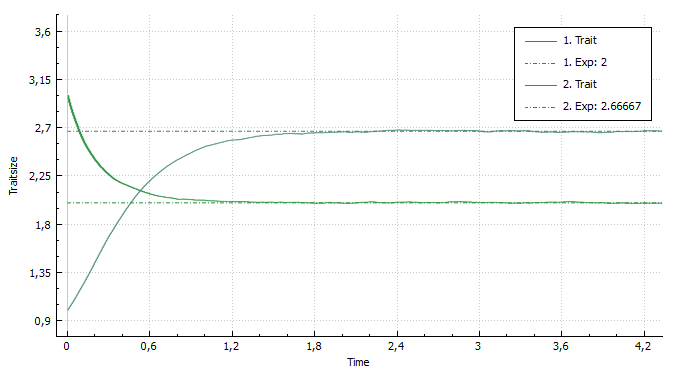
\includegraphics[width=1\linewidth]{./Pictures/BigKInstance_Equillibrium}
			\caption[Konvergenz_K=100000]{Konvergenz mit K=100000 und $ 15\cdot10^6 $ Spr"ungen}
			\label{Konvergenz_K=100000}
		\end{figure}
	
	\subsection{Der TSS Grenzwertprozess}
	Wie zuvor bei der LPA-Normalisierung erhalten wir TSS-Prozesse (Trait Substitution Sequence) als Grenzprozesse von BPDL-Prozessen mit gro"sen Populationen und seltenen Mutationen. Mit wachsendem K  soll f"ur die Mutationswahrscheinlichkeit durch die Vorschrift:
	\begin{align}
		\frac{1}{e^{cK}} \ll \mu_K \ll \frac{1}{K \log(K)}, \qquad \forall c > 0, \label{TSSMutation}
	\end{align}
%	\[  \frac{1}{e^{cK}} \ll \mu_K \ll \frac{1}{K log(K)}, \qquad \forall c > 0,  \] 
	eine schnellere Konvergenz gegen 0 stattfinden, als die Geburten pro fester Zeiteinheit gegen unendlich streben. D.h. mit wachsendem K werden Mutationen zunehmend seltener.\\ 
	Der TSS-Prozess ist ein besonders interessanter Grenzprozess des BPDL-Prozesses, weil es ihm m"oglich ist von einer monomorphen Population im Merkmal $ x $ zu einer anderen monomorphen Population mit Merkmal $ y $ zu springen, falls $ f(y,x) > 0 $ und $ f(x,y) < 0 $ (mehr dazu im Kapitel 7).\\
	In diesem Fall haben wir zu jeder festen Zeit h"ochstens 2 konkurrierende Merkmale. Diese Eigenschaft vereinfacht die Analyse des Prozesses sehr und ist der Wahl von $ \mu_K $ zu verdanken.\\
	\begin{figure}[H]
		\centering
		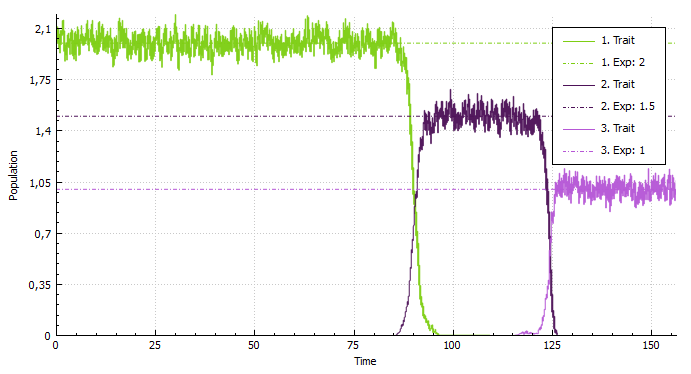
\includegraphics[width=1 \linewidth]{../BachelorArbeit/Pictures/TSS2_pure_small}
		\caption[TSS Prozess wechselnder Dominanz]{TSS Prozess mit: K = 1000 und $ 4 \cdot 10^6 $ Spr"ungen}
		\label{TSS_mitBPDLSimulator}
	\end{figure}
	\textbf{Frage:} Warum bietet $ \mu_K $ im Bereich (\ref{TSSMutation}) diese Eigenschaften?\\
	
	\textbf{Antwort:} Dank Freidlin und Wenzell \cite{freidlin2012random} erwarten wir, dass unsere dominante Spezies eine Zeit von der Ordnung $ \exp(cK) $ im Gleichgewicht bleibt. Schlie"slich k"onnen wir so kontrollieren wie lange uns eine dominante Spezies, die f"ur eine mutative Geburt in Frage kommt erhalten bleibt. Und dadurch, dass die Mutationen exponentiell verteilt sind, ben"otigt man eine Rate $ \mu_K \gg \frac{1}{e^{cK}} $ um eine Zeit von $ \exp(cK) $ nicht zu "uberschreiten, was die \underline{obere Schranke} rechtfertigt.\\
	Um die untere Schranke zu rechtfertigen, betrachten wir nun die Zeit, die ein Mutant braucht, um ein dominantes Merkmal aussterben zu lassen. Das wird uns die M"oglichkeit geben einer neuen Mutation so viel Zeit zu lassen bis das derzeit benachteiligte Merkmal ausgestorben ist.\\
	Angenommen es ereignet sich eine Mutation und der Mutant in $ y $ ist fitter ($ f(y,x) > 0, f(x,y) < 0 $), so wird es mit positiver Wahrscheinlichkeit eine Invasion ausl"osen (n"aheres dazu im Kapitel 7 - TSS Prozesse). Wenn man Branching Prozesse mit dem Lotka-Volterra System vergleicht, kommt man darauf, dass die ben"otigte Zeit zum Verdr"angen und Aussterben des urspr"unglich dominanten Merkmals von der Ordnung $ \log(K) $ ist.
%	Diese Invasion wird eine Zeit von der Ordnung $ \log(K) $ ben"otigen. Das l"asst sich folgern indem man Branching Prozesse mit 
%	
	Skaliert man nun noch zusätzlich die Zeit, so führt dies dazu, dass der Prozess ausreichend Zeit zwischen zwei Mutationen hat, um ein benachteiligtes Merkmal zu verdr"angen.
	Somit erlaubt uns die LPA-Annahme von einer deterministischen Populationsdynamik zwischen zwei Mutationen auszugehen \cite{raey}.\\
	
	
\clearpage
\section{Simulation}
In diesem Kapitel wird der Kern der Simulation algorithmisch n"aher untersucht. Dieser Kern besteht im Wesentlichen aus einem Sprung des BPDL-Prozesses.
Dabei wird zwischen der Implementierung und dem Pseudocode unterschieden, weil bei der Implementierung sorgf"altig auf die Trennung der Aufgabenbereiche geachtet wurde, welche sp"ater beim Verhaltenstest sehr wichtig werden und im 5. Kapitel weiter verwendet werden.\\
\textcolor{blue}{Die hier verwendete Vorgehensweise unterscheidet sich von der aus \cite{fournier2004microscopic}, weil wir ein System mit vielen Individuen und wenigen Merkmalen betrachten, was uns erm"oglicht, die individuellen Raten zu ber"ucksichtigen}.
	\subsection{Implementierung}
	Die Simulation durchl"auft mehrere Schritte bis ein vollst"andiger Sprung von $ \nu_t $ abgeschlossen ist. Hier wird beschrieben in welcher Reihenfolge welche Schritte durchlaufen werden und welche Aufgabe diese erf"ullen.\\
	Am Ende werden alle Funktionsaufrufe (Schritte) und Zusammenh"ange in Abbildung (\ref{fig:PseudoCodeForBThesis}) als ein Ablauf-Tiefen Diagramm illustriert.\\
	Im Code wird dabei objektorientiert mit Klassen und Objekten gearbeitet. Da diese Details nicht besonders von Interesse sind, wird eher ein heuristischer "Uberblick der Implementation gegeben. So kann hier z.B. angenommen werden, dass man mit der Variable \textit{Members[i]} Zugriff auf die Anzahl der Individuen des i-ten Merkmals hat, was im Code jedoch komplexer realisiert werden musste.\\
	
	\subsubsection{Raten berechnen}	
	Zun"achst m"ussen wir die Raten wissen, nach denen die exponentiellen Uhren gestellt werden, bevor ein Merkmal und Ereignis ausgew"ahlt werden kann.\\
	Die Todesrate setzt sich aus der intrinsischen Todesrate und der durch Wettbewerb zusammen und ist zu Beginn 0.\\
	
	Die folgende Funktion addiert die intrinsische Todesrate zur aktuellen Todesrate. Dabei wird direkt das Superpositionsprinzip genutzt, um die gesamte intrinsische Todesrate des Merkmals in "{}TotalDeathRate[i]"{} aufzuaddieren.
	\begin{algorithm}[H]
		\caption{addTotalIntrinsicDeathRateOf(TraitIndex: i)}
		\begin{algorithmic}[1]
			\Ensure{addiert zur Todesrate die intrinsische-Todesrate}
			\State TotalDeathRate[i] = DeathRate[i] $ \cdot $ Members[i]
		\end{algorithmic}
	\end{algorithm}
	Diese Funktion addiert die wettbewerbliche Todesrate zur aktuellen Todesrate.
	\begin{algorithm}[H]
		\caption{addTotalCompDeathRateOf(TraitIndex: i)}
		\begin{algorithmic}[1]
			\Ensure{addiert zur Todesrate die Wettbewerbs-Todesrate}
			\For{j=0 $ \to $ n-1}
				\State TotalDeathRate[i] += CompDeathRate[i,j] $ \cdot $ Members[i] $ \cdot $ Members[j];
			\EndFor
		\end{algorithmic}
	\end{algorithm}
	Auch wenn es vielleicht so erscheint, dass man zu stark trennt, ist es jedoch f"ur das verwendete Programmierkonzept entscheidend, dass jede Funktion nach M"oglichkeit eine genau Aufgabe hat \cite{martin2008clean}, weshalb diese beiden Funktionen getrennt wurden. Darauf wird etwas n"aher im n"achsten Kapitel eingegangen. \\
	Schlie"slich erfolgt aus obigem die Berechnung der Totalen Todesraten:
	\begin{algorithm}[H]
		\caption{calculateTotalDeathRates()}
		\begin{algorithmic}[1]
			\Ensure{berechnet die gesamten Todesraten aller Merkmale}
			\For{i=0 $ \to $ n-1}
				\State TotalDeathRate[i] = 0;
				\State addTotalIntrinsicDeathRateOf(i);
				\State addTotalCompDeathRateOf(i);
			\EndFor
		\end{algorithmic}
	\end{algorithm}
	Danach kommen wir zur Berechnung der Geburtsrate pro Merkmal. Auch hier sollten Mutationen und intrinsische Geburten gesondert berechnet werden. Zusammengefasst:
	\begin{algorithm}[H]
		\caption{calculateTotalBirthRates()}
		\begin{algorithmic}[1]
			\Ensure{berechnet die gesamten Geburtsraten aller Merkmale}
			\State $ \qquad $ $ \downarrow $ \textbf{intrinsische Geburtenrate} $ \downarrow $
			\For{i=0 $ \to $ n-1}
				\State TotalBirthRate[i] = Members[i] $ \cdot $ BirthRate[i] $ \cdot $ (1 - Mutation);
			\EndFor
			\State $ \qquad $ $ \downarrow $ \textbf{Mutationsraten} $ \downarrow $
			\For{i=1 $ \to $ n-2}
				\State TotalBirthRate[i] += Members[i-1] $ \cdot $ BirthRate[i-1] $ \cdot $ Mutation $ \cdot $ 0.5;
				\State TotalBirthRate[i] += Members[i+1] $ \cdot $ BirthRate[i+1] $ \cdot $ Mutation $ \cdot $ 0.5;
			\EndFor
			\State TotalBirthRate[0] += Members[1] $ \cdot $ BirthRate[1] $ \cdot $ Mutation $ \cdot $ 0.5;
			\State TotalBirthRate[n-1] += Members[n-2] $ \cdot $ BirthRate[n-2] $ \cdot $ Mutation $ \cdot $ 0.5;
		\end{algorithmic}
	\end{algorithm}
	 Jetzt sind wir bereit eine Funktion aufzurufen, die aus den vorher berechneten Geburts- und Todesraten pro Merkmal durch Superposition eine totale Eventrate berechnet, nach der wir eine exponentielle Uhr stellen k"onnen, die schlie"slich das Klingeln der Ersten aller Merkmalsuhren simuliert.
	 \begin{algorithm}[H]
 		\caption{calculateTotalEventRate()}
 		\begin{algorithmic}[1]
 			\Ensure{berechnet die Total Eventrate}
 			\State TotalEventRate = 0;
 			\For{i=0 $ \to $ n-1}
 				\State TotalTraitRate[i] = TotalBirthRate[i] + TotalDeathRate[i];
 				\State TotalEventRate += TotalTraitRate[i];
 			\EndFor
 		\end{algorithmic}
 	\end{algorithm}
 	Hier f"allt auf, dass wir auch die \textit{TotalTraitRate} oder Totale Merkmalsrate gespeichert haben. Diese repr"asentiert die gesamte Ereignisrate eines Merkmals.\\
 	Zum Schluss sollte es eine Funktion geben, die alle bisherigen Funktionen in der richtigen Reihenfolge ausf"uhrt und so die Berechnung aller Ereignisraten sichert:
 	\begin{algorithm}[H]
 		\caption{calculateEventRates()}
 		\begin{algorithmic}[1]
 			\Ensure{stellt sicher dass alle akutellen Raten berechnet wurden}
 			\State calculateTotalDeathRates();
 			\State calculateTotalBirthRates();
 			\State calculateTotalEventRate();
 		\end{algorithmic}
 	\end{algorithm}
	
	\subsubsection{Ereignis und Zeit bestimmen}
	
	Mit den zuvor berechneten Raten ist es jetzt einfach die Dauer bis zum n"achsten Ereignis zu bestimmen. An dieser Stelle verwende ich die Funktion \textit{rollExpDist(Parameter)} zum Ziehen einer exponentiell verteilten Zufallsvariable, die nicht weiter interessant ist und deshalb nicht erl"autert wird.
 	\begin{algorithm}[H]
 		\caption{sampleEventTime()}
 		\begin{algorithmic}[1]
 			\Ensure{Zieht die n"achste Ereigniszeit}
 			\State EventTime = rollExpDist(TotalEventRate);
 			\State Timeline += EventTime;
 		\end{algorithmic}
 	\end{algorithm}
 	Jetzt bleibt zu bestimmen, wem was passiert. Also welches Ereignis welches Merkmal treffen wird. Daf"ur wenden wir das Superpositionsprinzip in anderer Richtung an als bisher:\\
 	Zum Bestimmen des auserw"ahlten Merkmals beachten wir den Anteil der Merkmale an der Totalen Eventrate. Dieser ist klar erkennbar durch die Summe:
 	\[ \text{TotalTraitRate} = \sum_{i = 0}^{n - 1} \text{TotalTraitRate[i]} \]
 	Also hat das $ i-te $ Merkmal mit Wahrscheinlichkeit $ \frac{TotalTraitRate[i]}{TotalEventRate} $ das Ereignis ausgel"ost. Um also das verantwortliche Merkmal auszuw"ahlen, k"onnen wir eine Uniform verteilte Zufallsvariable ziehen und entscheiden welche der Merkmalsraten damit gemeint ist. Abbildung (\ref{SelectTrait}) illustriert den Auswahlprozess.
 	\begin{figure}[H]
		\centering
		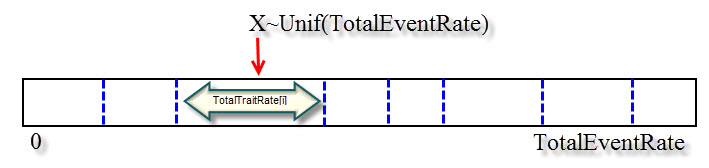
\includegraphics[width=1\linewidth]{./Pictures/SelectTrait}
		\caption[]{Auswahl des Merkmals nach Anteil an der TotalEventRate}
		\label{SelectTrait}
	\end{figure}
	Im Code wird daf"ur iterativ gepr"uft, ob "{}X $ \sim $ Unif(TotalEventRate)"{} im ersten Intervall der L"ange TotalTraitRate[0] liegt. 
	\begin{itemize}
		\item[] Falls ja, so wird dieses Merkmal gew"ahlt und die Funktion wird verlassen.
		\item[] Falls nicht, so wird das Merkmal $ 0 $ aus den relevanten Merkmalen entfernt und X wird um die Intervallänge TotalTraitRate[0] reduziert, um schlie"slich erneut mit dem ersten relevanten Intervall verglichen zu werden (jetzt TotalTraitRate[1]). Auf diese Weise n"ahert man sich immer weiter dem getroffenen Merkmal:
	\end{itemize}
	\begin{algorithm}[H]
 		\caption{choseTraitToChange()}
 		\begin{algorithmic}[1]
 			\Ensure{w"ahlt ein Merkmal zum "Andern aus}
 			\State X = rollUnifDist(TotalEventRate);
 			\For{i=0 $ \to $ n-1}
 				\If{X $ \le $ TotalTraitRate[i]}
 					\State ChosenTrait = i;
 					\State return;
 				\EndIf
 				\State X -= TotalTraitRate[i];
 			\EndFor
 		\end{algorithmic}
 	\end{algorithm}
 	Auf die selbe Weise wird entschieden, welches Ereignis eintrifft und anschlie"send in \textit{isBirth} gespeichert. Da wir hier jedoch nur Geburt und Tod zur Auswahl haben, w"urde sich nat"urlich eine Bernoulli verteilte Zufallsvariable ergeben mit:
 	\[ \text{isBirth} \sim \text{Ber(TotalBirthRate[ChosenTrait])} \]
 	Im Code wurde \textit{isBirth} folgenderma"sen gezogen:
	\begin{algorithm}[H]
 		\caption{choseEventType()}
 		\begin{algorithmic}[1]
 			\Ensure{w"ahlt ein Ereignis f"ur das entsprechende Merkmal aus}
 			\State X = rollUnifDist(TotalTraitRate[ChosenTrait]);
 			\If{X $ \le $ TotalBirthRate[ChosenTrait]}
 				\State isBirth = true;
 			\Else
 				\State isBirth = false;
 			\EndIf
 		\end{algorithmic}
 	\end{algorithm}
 	Danach muss noch das Ereignis aus Alg. 9 auf das Merkmal aus Alg. 8 angewendet werden.
	\begin{algorithm}[H]
 		\caption{executeEventTypeOnTrait()}
 		\begin{algorithmic}[1]
 			\Ensure{wendet das gew"ahlte Ereignis auf das gew"ahlte Merkmal an}
 			\State X = rollUnifDist(TotalTraitRate[ChosenTrait]);
 			\If{isBirth}
 				\State Members[ChosenTrait] += 1;
 			\EndIf
 			\If{$ \neg \text{isBirth} $ \& Members[ChosenTrait] $ > $ 0}
 				\State Members[ChosenTrait] -= 1;
 			\EndIf
 		\end{algorithmic}
 	\end{algorithm} 	
 	Zum Schluss wird noch eine Funktion erstellt, welche das Ausf"uhren eines Ereignisses in richtiger Reihenfolge realisiert und in einem Schritt aus gegebenen Raten die eine Ver"anderung der Population durchf"uhrt.
 	\begin{algorithm}[H]
 		\caption{changeATrait()}
 		\begin{algorithmic}[1]
 			\Ensure{l"asst ein Ereignis ein Merkmal treffen}
 			\State choseTraitToChange();
 			\State choseEventType();
 			\State executeEventTypeOnTrait();
 		\end{algorithmic}
 	\end{algorithm} 
	Aus diesen 3 wesentlichen Schritten
	\begin{itemize}
		\item Raten berechnen
		\item Ereigniszeit ziehen
		\item Ereignis eintreten lassen
	\end{itemize}
	kann schlie"slich eine sehr "ubersichtliche Funktion konstruiert werden, die einen kompletten Sprung des Prozesses durchf"uhrt.
	\begin{algorithm}[H]
 		\caption{makeEvolutionStep()}
 		\begin{algorithmic}[1]
 			\Ensure{l"asst ein Ereignis ein Merkmal treffen}
 			\State calculateEventRates();
 			\State sampleEventTime();
 			\State changeATrait();
 		\end{algorithmic}
 	\end{algorithm}
	 	
	\subsubsection{"Ubersicht}
	Hier ist eine "Ubersicht aller Funktionen, ihrer Reihenfolge und Aufruftiefe. \\
	Die Funktionen wurden auf Englisch beschrieben, weil sie damit eine Referenz zu der im Quellcode beschriebenen Funktion darstellen. Z.B. "{}make one evolution step"{} verweist auf die Funktion "{}makeEvoultionStep"{}, oder "{}calculate event rates"{} $ \to $ "{}calculateEventRates"{} etc.
	\begin{figure}[H]
		\centering
		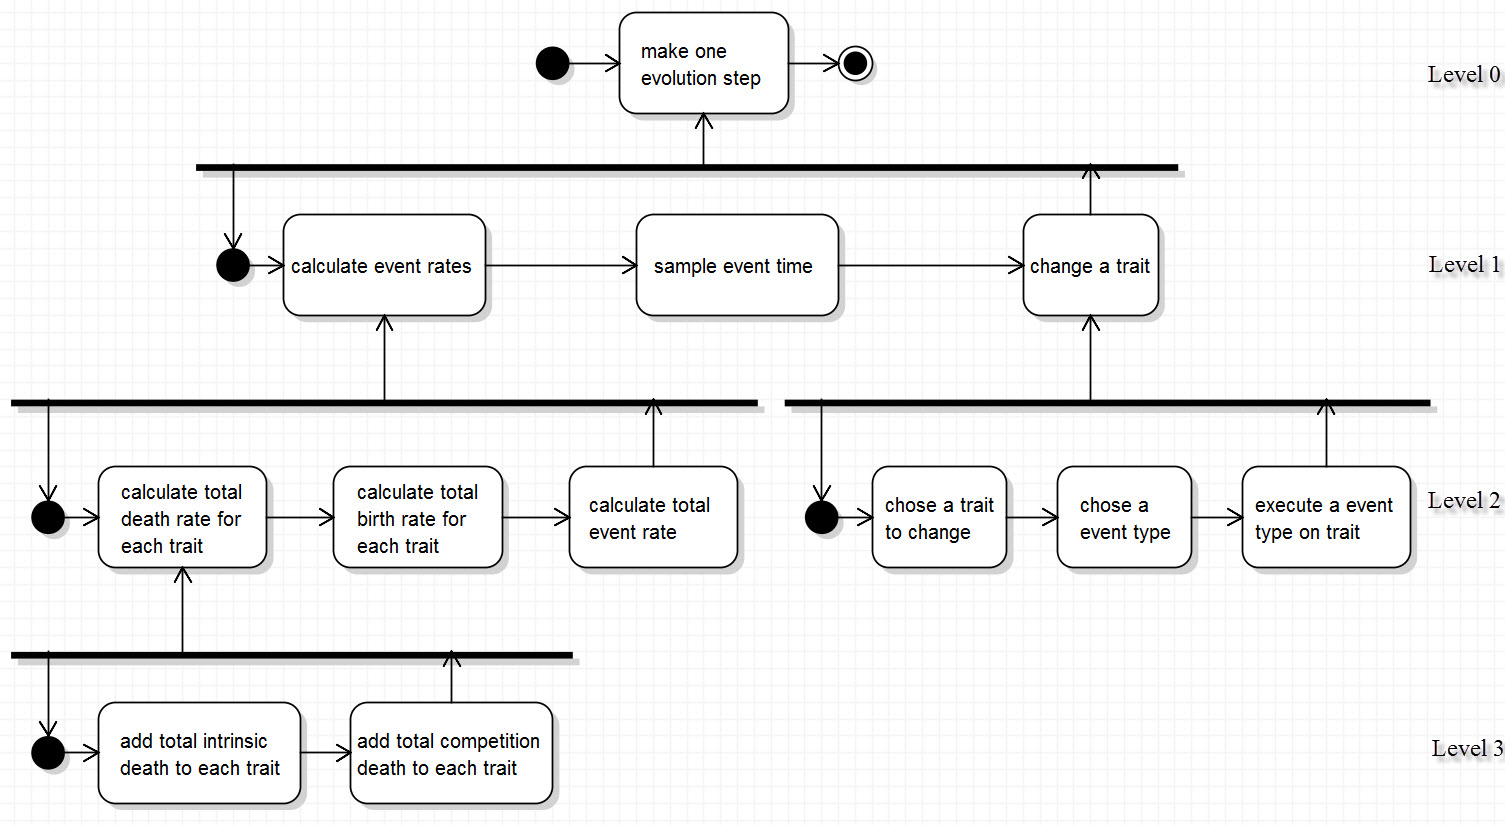
\includegraphics[width=1\linewidth]{../UMLs/PseudoCodeForBThesis}
		\caption{Diagramm mit Funktionsaufrufen und ihren Tiefenebenen}
		\label{fig:PseudoCodeForBThesis}
	\end{figure}
	
	\subsection{Pseudocode}
	Nat"urlich l"asst sich der Ablauf eines Sprunges auch durch Pseudocode in eine Funktion "{}makeEvoultionStep"{} zusammenfassen.\\
	Im Pseudocode finden sich in blau einige Verweise auf die zuvor beschriebene Implementierung.
	
	\begin{algorithm}[H]
		\caption{makeEvolutionStep() - Part 1}
		\begin{algorithmic}[1]
			\Ensure{A full evolution Step happened}
			\Require $ t, X = \{0,\dots, n-1\} $
			\For{ $ x \in X $ }\Comment{$ \downarrow $ \textcolor[rgb]{0,0,0.55}{calculateEventRates}() $ \downarrow $}
				\State $  D(x) := n_t(x) \cdot \left( d(x) + \sum_{y \in X} c(x,y) \cdot n_t(y) \right) $
				\State $ B(x) := \underbrace{b(x) \cdot (1 - \mu) \cdot n_t(x)}_{arteigene}  $
				\If{$ x > 0 $}
					\State $ B(x) += \underbrace{b(x-1)\cdot n_t(x-1)}_{Mutation Links} \cdot \frac{\mu}{2} $
				\EndIf
				\If{$ x < n-1 $}
					\State $ B(x) += \underbrace{b(x+1)\cdot n_t(x+1)}_{Mutation Rechts} \cdot \frac{\mu}{2} $
				\EndIf
				\State $ TotalTraitRate(x) = B(x) + D(x) $
			\EndFor
			\State $ TotalEventRate := \sum_{x \in X} TotalTraitRate(x) $
			\State sample $ Z \sim exp(TotalEventRate) $ \Comment{$\downarrow $ \textcolor[rgb]{0,0,0.55}{sampleEventTime}() $ \downarrow $} 
			\State $ t += Z $
			
			\State sample $ Y \sim U(0,TotalEventRate) $ \Comment{$ \downarrow $ \textcolor[rgb]{0,0,0.55}{choseTraitToChange}() $ \downarrow $}
			\For{$ x \in X $}
				\If{$ Y \le TotalTraitRate(x) $}
					\State $ ChosenTrait := x $
					\State break
				\EndIf
				\State $ Y -= TotalTraitRate(x) $
			\EndFor 
			
			\State sample $ Y \sim U(0,TotalTraitRate(ChosenTrait)) $
			\If{$ Y \le B(ChosenTrait) $} \Comment{$ \downarrow $ \textcolor[rgb]{0,0,0.55}{choseEventType()} $ \downarrow $}
				\State isBirht := true
			\Else
				\State isBirth := false
			\EndIf
			\If{isBirth} \Comment{$ \downarrow $
				\textcolor[rgb]{0,0,0.55}{executeEventTypeOnTrait()} $ \downarrow $}
				\State $ n_t(ChosenTrait) += 1 $
			\Else
				\If{$ n_t(ChosenTrait) \ge 0 $}
					\State $ n_t(ChosenTrait) -= 1 $
				\EndIf
			\EndIf
		\end{algorithmic}
	\end{algorithm}
	
	\subsection{Optimierung f"ur viele Merkmale}
	F"ur eine Simulation ist klar, dass in Abh"angigkeit der Spr"unge (wenn auch hoher) linearer Aufwand zu erwarten ist.\\
	Zwar ist der nachvollziehbar am Modell gehalten worden, jedoch ist durch die Wettbewerbsrate ein quadratischer Aufwand in der Anzahl der Merkmale nicht vermieden worden.\\
	In unserer Situation werden wir immer eine "uberschaubare Menge an Merkmalen haben, aber der Nutzen meiner Optimierung ist bereits ab einem Merkmal sp"urbar (praktisch wurde er erst ab dem 2. gemessen, vgl. Abb. \ref{Test Results}).\\
	Nach meinen Tests, die sp"ater im Kapitel "{}Verhaltenstest"{} eingef"uhrt werden, ergab sich der gr"o"ste zeitliche Aufwand in der Berechnung der Raten (genauer der Todesraten), was auch zu erwarten war.\\
	Diese Optimierung vermeidet es die Raten komplett neu zu berechnen und m"ochte sie stattdessen anpassen. \\
	Dazu werden die Raten nicht zu Beginn berechnet wie zuvor in Algorithmus 12 "{}makeEvolutionStep()"{} in der 1. Zeile. Als erstes wird mit den aktuellen Raten eine Ereigniszeit gezogen "{}sampleEventTime()"{} und anschlie"send ein Ereignis ausgel"ost "{}changeATrait()"{}, welches es erm"oglicht die n"achsten Raten anzupassen "{}adjustNewEventRates()"{}.\\
	Daf"ur wird zun"achst unterschieden, ob ein Tod oder eine Geburt eingetreten ist. Das l"asst sich leicht mit der in Algorithmus 9 erw"ahnten "{}isBirth"{} Variable entscheiden.\\
	Angenommen es ereignet sich eine Geburt. Damit kann zusammen mit dem ausgew"ahlten Merkmal "{}chosenTrait"{} folgende Anpassungen gemacht werden:
	\begin{itemize}
		\item Die \textbf{intrinsische Todesrate} von "{}chosenTrait"{} wird um  die des geborene Individuums erh"oht:\\ 
		TotalDeathRate[chosenTrait] += DeathRate[chosenTrait];
		\item Die \textbf{Todesrate durch Wettbewerb} wird bei jedem Merkmal um das geborene Individuum erh"oht:\\
		TotalDeathRate[i] += CompDeathRate[i][chosenTrait]; $ \qquad \forall \text{ i} \in X $
		\item Die \textbf{Geburtsraten} werden genauso wie die Todesraten behandelt:\\
		TotalBirthRate[chosenTrait] += BirthRate[chosenTrait];
		\item Und passend die Mutationsraten:\\
		TotalBirthRate[i] += Mutation $ \cdot $ 0.5 $ \cdot $ BirthRate[chosenTrait]; \\
		$\forall \text{ i } \sim \text{ chosenTrait} $
		\item Zum Schluss noch die Totale Ereignisrate:\\
		Hier kann man nicht vermeiden alle Totalen Raten erneut auszurechnen.
	\end{itemize}
	Man erkennt, dass hier keine quadratische Abh"angigkeit der Merkmale mehr zu finden ist.
	
	\subsection{Normalisierung}
	Vielleicht ist aufgefallen, dass weder in der Implementierung noch im Pseudocode die Normalisierung erw"ahnt wurde. Diese Option wurde vom Programmkern getrennt, weil sie den evolution"aren Mechanismus nicht beeinflusst, sondern nur die Sichtweise ver"andert.\\
	Um das zu realisieren wurde an zwei Stellen Ver"anderungen vorgenommen.
	\begin{itemize}
		\item [\textbf{1.}] Unmittelbar nach dem Lesen dem Einlesen der Parameter, wurde sowohl die Wettbewerbsrate durch K geteilt als auch die Startpopulation um K hoch skaliert. Auf diese Weise kann der Programmkern ohne Kenntnis eines K die Evolution durchf"uhren.\\ 
		Dadurch l"asst sich ein Prozess einfach durch wachsendes K verfeinern, ohne R"ucksicht auf anzupassende Parameter zu nehmen und man kann mit wachsendem K die Konvergenz wie in Abbildung \ref{Konvergenz_K=100000} verfolgen.
		\item [\textbf{2.}] Zuletzt geht es darum, dass die Ergebnisse zwar ohne R"ucksicht auf ein vorhandenes K berechnet wurden, aber die Darstellung sollte nat"urlich reskaliert erfolgen ($ \nu_t^K = \frac{\nu_t}{K} $). Deswegen ist es au"serhalb des Programmkerns nur "uber einen sogenannten "{}getter"{} (eine spezielle Zugriffsfunktion) m"oglich auf die Mitglieder eines Merkmals zuzugreifen. Dieser "{}getter"{} liefert stehts den reskalierten Wert zur"uck.\\
	\end{itemize}
	
	\subsubsection{Sehr viele Spr"unge}
	Gerade bei der Normalisierung wird es mit wachsendem K notwendig besonders viele Spr"unge zu machen. Die Anzahl der Spr"unge "ubersteigt schnell das Fassungsverm"ogen eines Arrays.	Um auch mehr als 100 Millionen Punkte speichern zu k"onnen, wurden zwei L"osungen implementiert.\\
	\begin{itemize}
		\item[\textbf{1.}] Die "{}erweiterten Spr"unge"{} sind eine L"osung, die zur Zeit angewendet wird. Zu Beginn der Simulation wird anhand der maximalen Iterationen entschieden wie viel Speicher ben"otigt wird und setzt eine "{}Jumps"{} Variable. Diese "{}Jumps"{} Variable enth"alt die Anzahl der Spr"unge bis ein Punkt gespeichert wird. So wird bei 100 Millionen Iterationen nur jeder zehnte Punkte gespeichert. \\
		\item[\textbf{2.}] Eine weitere L"osung ist die "{}storePoint()"{} Funktion. Sie erstellt zu Beginn der Rechnung eine Datei und h"angt immer weiter Punkte an bis die Berechnung vorbei ist.\\
		Schlie"slich wird die Graphklasse einzeln jeden Punkt am Graphen anh"angen.\\ 
		Diese Variante ist implementiert und wurde getestet. Sie ist auch in einem Unit Test enthalten, der aber nicht im Kapitel 6 erl"autert wird.
	\end{itemize}

	
	
\clearpage	
\section{Das Programm}
In diesem Kapitel werden die Programme und ihre Entwicklung vorgestellt. Dabei wird darauf eingegangen, welche M"oglichkeiten es gibt eine GUI zu entwickeln, welche Architektur im Programm verwendet wurde, welcher Codestil und wie das Layout der Programme gew"ahlt wurde und zu bedienen ist.\\
Zun"achst sei gesagt, dass die Programme zum Zeitpunkt der Erstellung der Bachelorarbeit noch nicht v"ollig fertig gestellt sind. Es gibt noch "uberfl"ussige Funktionen im TSS Simulator und noch einige W"unsche zur erweiterten Verwendung des Programms. 

	\subsection{GUI - Entwicklung}
	Ziel war es, ein Programm mit einer graphischen Oberfl"ache in C++ zu schreiben. Nach \cite[14 - Grafische Benutzungsschnittstellen]{breymann2011c++} kennt Standard C++ keine Elemente f"ur grafische Benutzungsoberfl"achen (englisch \textit{graphical user interfaces - GUI}). Weil es f"ur unseren Fall jedoch nicht wegzudenken ist, wird hier kurz vorgestellt, warum welche Variante der GUI-Programmierung ausgew"ahlt werden sollte und welche es gibt.\\
	
	\textbf{MFC}\\
	Sehr bekannt sind die Microsoft Foundation Classes (MFC) bzw. ihre Nachfolger in .NET f"ur Windows Betriebssysteme. Aber genau hier liegt bereits das Problem. In unserem Fall wurden die Programme f"ur zwei Mitarbeiter entwickelt, welche jeweils MAC verwendeten, an einem Institut, welches "uberwiegend mit Ubuntu arbeitet. Deswegen kam MFC nicht in Frage.\\
	
	\textbf{$ \text{GTK}_+ $ }(the GIMP Toolkit)\\
	Das ist eine weitere Bibliothek zur Erstellung von GUI's. Sie wurde haupt-sächlich f"ur GIMP, ein m"achtiges Bildbearbeitungsprogramm, entwickelt. $ \text{GTK}_+ $ wird zur Entwicklung des GNOME-Desktops benutzt, welche auf vielen Linux Systemen zu finden sind. Aber auch dazu gibt es eine bessere Alternative.\\
	
	\textbf{Qt}\\
	Die portable Qt-Bibliothek ist sehr bekannt und l"asst sich sehr einfach auf Windows-, Mac- und Unix Betriebssysteme portieren. Die aus manchen Linux-Systemen bekannte Benutzungsoberfl"ache KDE wird mit Qt entwickelt. Damit bietet sich Qt bereits jetzt als eine gute Option zur Entwicklung f"ur alle Betriebssysteme an.\\
	Hinzu kommen noch viele weitere Vorteile, wie die gro"se Auswahl an Hilfsprogrammen und Bibliotheken, die sehr ausführliche Dokumentation oder dass es eine Oben Source Software ist.\\
	"{}Zusammengefasst: Qt ist die ausgereifteste und umfangreichste Open Source Software f"ur die portable Entwicklung grafischer Benutzungsoberfl"achen mit C++"{}\cite[S.452]{breymann2011c++}

	\subsection{Architektur und Module}
	\textcolor{blue}{Modul hei"st m"oglichst unabh"angige Sammlung [...]}\\
	Zuerst m"ochte ich die grobe Architektur des Programmcodes vorstellen. Diese kann in drei Module zusammengefasst werden, welche m"oglichst wenige Schnittstellen untereinander verwenden und damit viel Unabh"angigkeit bieten.
	
	\begin{itemize}
		\item [\textbf{1.}] "{}Population Kernel"{}\\
		Der Programmkern besteht aus dem "{}Population Kernel"{}, welcher ausschlie"slich f"ur die Berechnungen zust"andig ist. Hier werden keine historischen Daten gespeichert, womit dieser Bereich immer nur die Daten der Population zur aktuellen Berechnung bereit h"alt. Also enth"alt dieser nur eine Sammlung von Funktionen, die das Modell befragen k"onnen.\\
		Die einzige Klasse dieses Moduls, mit der eine Kommunikation nach au"sen m"oglich ist, ist der "{}TraitEventManager"{}, der wie der Name schon sagt die Ereignisse und Merkmale verwaltet (Abb. \ref{Module und Klassen}, rechts).\\
		Das Besondere an diesem Bereich ist, dass er mit Standard C++11 implementiert wurde und somit "uberall wiederverwendbar ist. Er ist leicht zu ver"andern und sehr flexibel, weshalb man z.B. einen anderen "{}Population Kernel"{}, der ein anderes Modell beschreibt, ohne Ver"anderungen an anderen Modulen vornehmen zu m"ussen, mit unserem ersetzten kann.\\
		Nat"urlich m"usste der neue Kernel weiterhin die Funktion "{}makeEvoultionStep"{} implementieren.
		\item [\textbf{2.}] "{}Graph Management"{}\\
		Der zweite Bereich organisiert alle Daten, die die Simulation anfragen kann. Hier liegt der eigentliche Speicher und die Kommunikation zwischen GUI und Algorithmus.\\
		Es ist eine Art Hilfsklasse, die eine Kommunikation zwischen den Modulen erm"oglicht. Zu diesem Zweck wurde hier bereits die Qt-Bibliothek verwendet, um Daten f"ur die GUI abholbereit anzubieten.\\
		Sie erh"alt die W"unsche des Users in Form von Anweisungen aus dem "{}GUI"{} und verwendet die M"oglichkeiten des "{}Population Kernel"{}, um entsprechende Daten abrufbereit zu erstellen.
		\item [\textbf{3.}] "{}GUI"{}\\
		Das letzte und unflexibelste Modul umfasst die grafische Benutzungsoberfl"ache. Hier kommen zwei wichtige Klassen zum Einsatz.\\
		Die erste "{}MainWindow"{} ist das Hauptfenster, in dem der Nutzer die Parameter festlegen und wenn alles stimmt auch die Simulation starten kann. Um f"ur die Analyse der Ergebnisse m"oglichst viel "Ubersicht zu haben, verwendet das Hauptfenster eine weitere Klasse "{}PlotWindow"{}, welche ein extra Fenster mit Graphen "offnet (Plot-Fenster).\\
		Wie man vermuten kann, wird hier bereits etwas zum Darstellen eines Graphen und fast ausschlie"slich Qt-Programmierung verwendet.\\
		Dieses Plot-Fenster verwendet ein "{}GraphClass"{} Objekt, um einen Graphen erstellen zu k"onnen. Nat"urlich ist es f"ur die Verwendung der Daten selber verantwortlich.
	\end{itemize}	
 	
 	Die folgende Abbildung \ref{Module und Klassen} stellt zusammenfassend die obigen Module und die Klassenhierarchie dar:
	\begin{figure}[H]
		\centering
		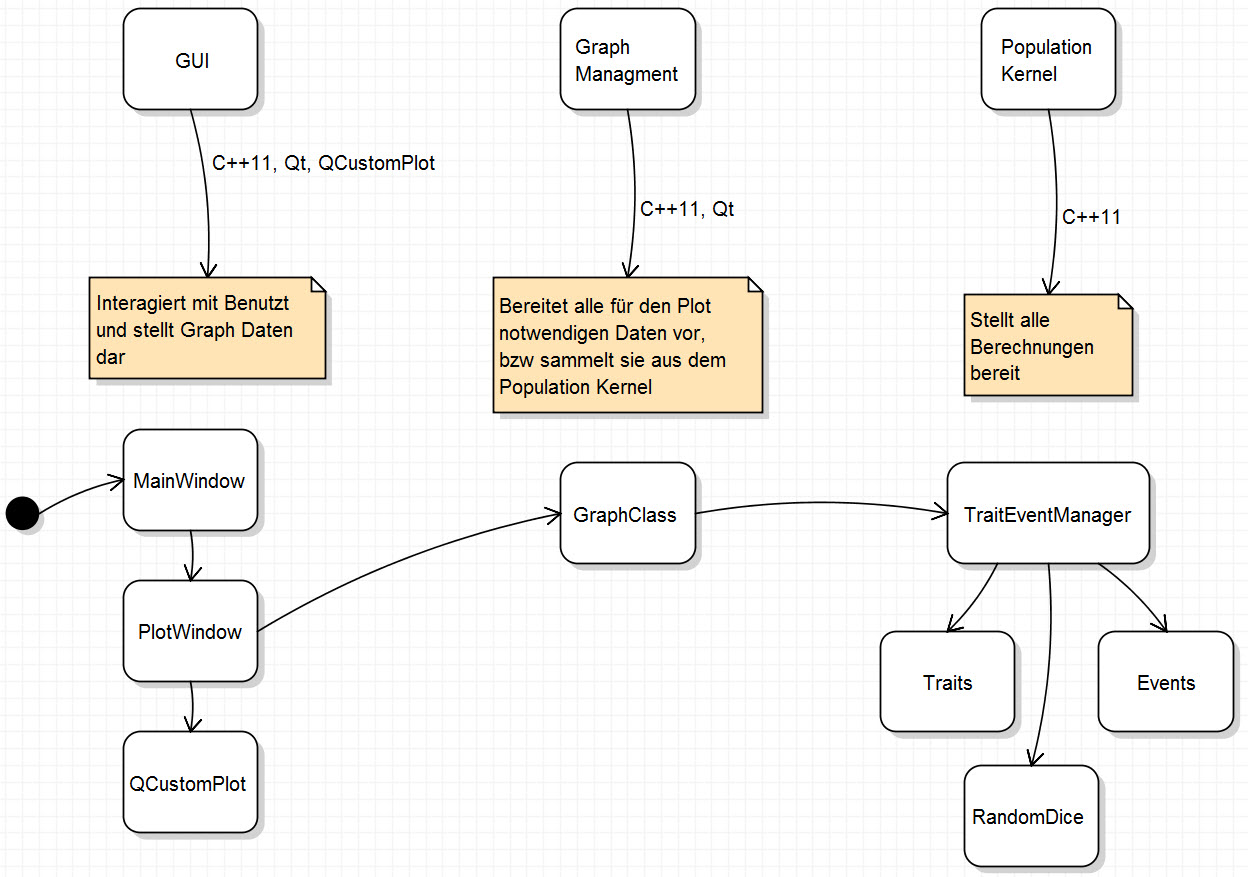
\includegraphics[width=1 \linewidth]{./Pictures/Bild_Module}
		\caption[Module]{Arbeitsmodule und Klassenabhängigkeiten}
		\label{Module und Klassen}
	\end{figure}	
		
	\subsection{Flexibilit"at und agile Softwareentwicklung}
	Die Idee der getrennten Aufgabenbereiche geht darauf zurück, dass eine möglichst große Unabhängigkeit zwischen Arbeitsschritten notwendig ist, um das Programm flexibel zu halten und sogenannten "{}Coderot/Softwareerosion"{} (faulen Code) zu verhindern \cite{martin2008clean}. \\
	Dieser bezeichnet die zunehmende Entropie einer Software.\\ 
	Das hei"st sie führt mit zunehmender Weiterentwicklung der Software zu einer Verringerung der Leistung, Erschwernissen bei der Anpassbarkeit bzw. Flexibilit"at und in zunehmendem Ma"se zu undefiniertem Verhalten.\\
	In der Softwareentwicklung ist undefiniertes Verhalten schwer zu behandeln, da man keine Fehler beim Compilieren oder Ausf"uhren erh"alt. Es wird lediglich ein nicht nachvollziehbares Verhalten des Programms festgestellt, welches sich im obigen Falle nur noch sehr schwer im Code eingrenzen l"asst.\\
	
	Au"serdem wurde darauf geachtet, dass jede Klasse nur eine m"oglichst fest definierte Aufgabe zu erf"ullen hat. In einer Klasse sollten lediglich Funktionen vorhanden sein, die zur Erf"ullung dieser Aufgabe beitragen. Dieses Prinzip tr"agt den Namen "{}Single-Responsability-Prinzip"{} und wurde von Robert C. Martin in \cite{Martin:2003:ASD:515230} eingef"uhrt. Die dort beschriebene "{}Agile Softwareentwicklung"{} fand auch Anwendung bei der Neuorganisation von Zielen und W"unschen mit Loren Coquille und Martina Baar, wird aber hier nicht weiter erl"autert.
	
	\subsection{Layout}
	Hier wird die Oberfl"ache des Programms vorgestellt.
	\subsubsection{Lesen und Anzeigen von Parameter}
	Die Bedienung des Programms sollte das Lesen und Anzeigen der Merkmals-Parameter bereitstellen. Da es viele Parameter gibt und die Anzahl der Parameter quadratisch mit der Anzahl der betrachteten Merkmale steigt, bietet sich das Lesen aus zuvor erstellten Dateien an.\\
	Dabei werden die Daten aus den Dateien in folgender Reihenfolge zeilenweise ausgelesen (Abbildung \ref{Parameter}):
	\begin{itemize}
		\item $ m $: Anzahl der Merkmale
		\item $ K $: Parameter
		\item $ \mu $: Mutationswahrscheinlichkeit
		\item $ c(1,1) \text{ } \dots \text{ } c(1,m) $: 1. Zeile der Wettbewerbsraten \\
			$ \vdots $\\
			$ c(m,1) \text{ } \dots \text{ } c(m,m) $: m.te Zeile der Wettbewerbsraten 
		\item $ n_0(1) $: Populationsgr"o"se des 1. Merkmals: \\
			$ \vdots $\\
			$ n_0(m) $: Populationsgr"o"se des m. Merkmals: 
		\item $ b(1) $: Geburtenrate des 1.Merkmals\\
			$ \vdots $\\
			$ b(m) $: Geburtenrate des m.Merkmals
		\item $ d(1) $: Todesrate des 1.Merkmals\\
			$ \vdots $\\
			$ d(m) $: Todesrate des m.Merkmals
	\end{itemize}
	
	\begin{center}
	\begin{minipage}{0.15\textwidth}
		\begin{figure}[H]
			\centering
			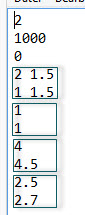
\includegraphics[width=1\linewidth]{./Pictures/Parameter}
			\caption[Parameter]{Datei}
			\label{Parameter}
		\end{figure}
	\end{minipage}
	$ \quad $
	\begin{minipage}{0.6\textwidth}
		Dabei wird $ \mu $ und $ c $ nat"urlich ohne Skalierung mit $ K $ angegeben. Die Gr"unde daf"ur wurden im Kapitel 4.4 Normalisierung beschrieben.\\
		
		Nebenstehend in Abb. \ref{Parameter} sieht man ein Beispiel einer Instanz mit zwei Merkmalen, $ K = 1000 $, $ \mu = 0 $ usw., wobei die Markierungen die Wettbewerbsmatrix, die Startpopulation, die Geburtenraten und die Todesraten enthalten.\\
	\end{minipage}
	\end{center}
	
	Das Programm muss also die Eingabe eines g"ultigen Dateinamens fordern bevor eine Simulation gestartet werden kann. Deshalb werden bis zum Zeitpunkt gelesener Parameter alle nicht relevanten Schaltfl"achen deaktiviert und nur ausgegraut angezeigt (Abbildung \ref{MainWindow_Start}, gelb markiert).\\
	Sobald man einen Namen in das einzige m"ogliche Feld eingegeben hat, kann man zwischen den Schaltfl"achen "{}load File"{} und "{}create File"{} w"ahlen (Abbildung \ref{MainWindow_Start}, rot markiert).\\
	
	\begin{figure}[H]
		\centering
		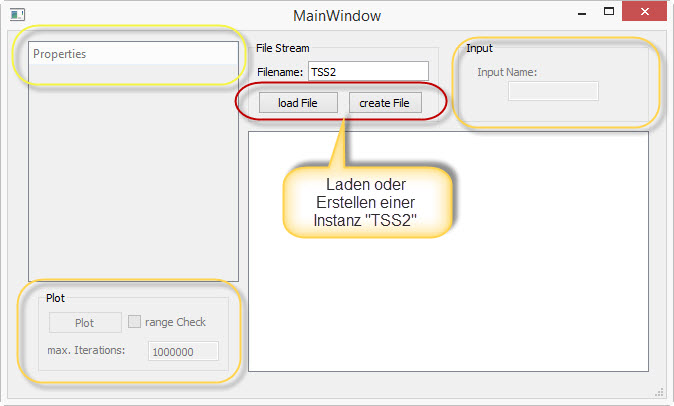
\includegraphics[width=1\linewidth]{./Pictures/MainWindow_Start}
		\caption[Startwindow]{MainWindow nach dem Start}
		\label{MainWindow_Start}
	\end{figure}
	Wie schon zuvor erw"ahnt, ist dem Programm vorab unbekannt, welchen Umfang die gelesenen Parameter haben werden, weshalb die Entscheidung der Darstellung auf eine Baumstruktur fiel.\\
	Sie hat bei der Initialisierung immer den selben Umfang (Abbildung \ref{Baumstruktur_geschlossen}) und der gew"unschte Ast l"asst sich einfach erweitern (Abbildung \ref{Baumstruktur_offen}).
	\begin{center}
	\begin{minipage}{0.45\textwidth}
		\begin{figure}[H]
			\centering
			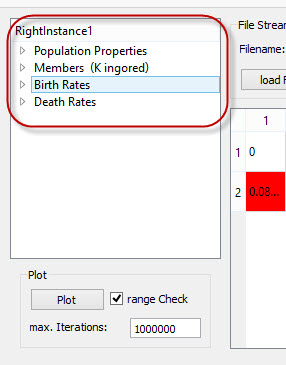
\includegraphics[width=1\linewidth]{./Pictures/MainWindow_ParameterBaum_zu}
			\caption[MainWindow_Parameter]{Baumstruktur - geschlossen}
			\label{Baumstruktur_geschlossen}
		\end{figure}
	\end{minipage} $ \quad $
	\begin{minipage}{0.45\textwidth}
		\begin{figure}[H]
			\centering
			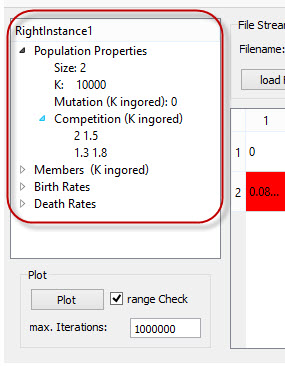
\includegraphics[width=1\linewidth]{./Pictures/MainWindow_ParameterBaum_offen}
			\caption[MainWindow_Parameter]{Verzweigte Baumstruktur - geöffnet}
			\label{Baumstruktur_offen}
		\end{figure}
	\end{minipage}
	\end{center}
		
	\subsubsection{Schreiben neuer Testinstanzen}
	Die letzte Herausforderung bestand darin, eine Instanz durch das Programm geleitet erstellen zu können. Während diese Aufgabe bei einer Konsolenanwendung (bekannt aus den klassischen c Programmen) denkbar einfach mit "{}printf"{} und "{}scanf"{} erledigt werden konnten, st"o"st man hier auf das Problem der sogenannten "{}Ereignisgesteuerten Programmierung"{} \cite{breymann2011c++}.\\
	W"ahrend zuvor die Reihenfolge der Programmschritte vorbestimmt war, so gilt das nicht mehr f"ur graphische Benutzungsoberfl"achen. Einfach weil die Reihenfolge der Interaktionsschritte eines Benutzters, z.B. Anklicken oder Mausbewegung, nicht vorhersehbar ist und daher auch nicht die Reihenfolge der auszuf"uhrenden Programmschritte.\\
	Es geht also darum, Funktionen zu schreiben, die nicht an anderer Stelle vom Programm, sondern bei Eintreffen eines Ereignisses aufgerufen werden und die gew"unschte Reaktion liefern.\\
	Da diese feste Reihenfolge jedoch beim Schreiben neuer Testinstanzen unbedingt eingehalten werden muss, wurde f"ur diesen Fall nur eine Eingabem"oglichkeit offen gelassen (Abbildung \ref{fig:MainWindow_createFile}) und die Parameter der Reihe nach abgefragt. Die Eingabeaufforderung wird durch das "uber der Textbox liegende Label gegeben vermittelt und dient dem Programm als "{}Lesezeichen"{}, um den gelesenen Parameter einzuordnen.\\
	\begin{figure}[H]
		\centering
		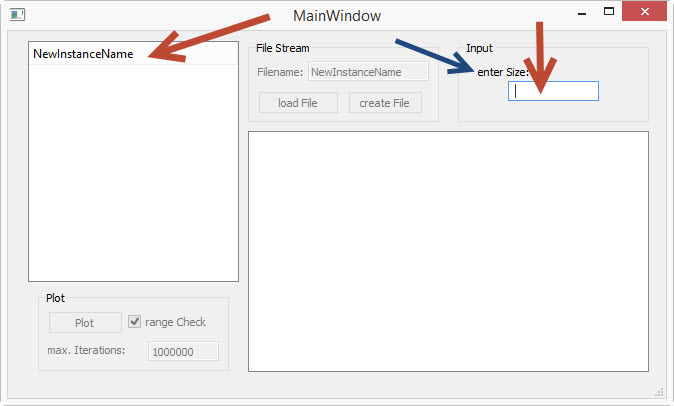
\includegraphics[width=1\linewidth]{./Pictures/MainWindow_createFile}
		\caption[erstelle Datei]{Nach Klick auf "{}create File"{} werden die neuen Parameter einzeln abgefragt}
		\label{fig:MainWindow_createFile}
	\end{figure}
	
	Nach erfolgreichem Einlesen aller Parameter wird die neue Instanz geladen und nebenstehend angezeigt.
	
	\begin{figure}[H]
		\centering
		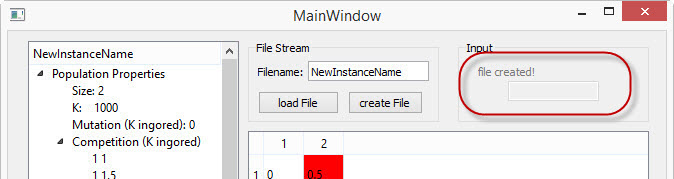
\includegraphics[width=1\linewidth]{./Pictures/MainWindow_FileCreated}
		\caption[Datei erstellt]{Nach Eingabe des letzten Parameters}
		\label{fig:MainWindow_FileCreated}
	\end{figure}
	
	\subsubsection{Darstellung des Graphen}
	Nach dem Erstellen oder Laden einer Testinstanz ist es m"oglich die Simulation zu starten. Das erkennt man an dem aktivierten "{}Plot"{} Bereich (vgl. Abb. \ref{MainWindow_Start}, zu \ref{Baumstruktur_geschlossen}, \ref{Baumstruktur_offen}, \ref{fig:MainWindow_FileCreated}) links unten.\\
	Wie man schon auf vielen Abbildungen zuvor beobachten kann, gibt es im "{}Plot"{} Bereich ein Eingabefeld mit dem Titel "{}max. Iterations:"{} und ein Auswahlk"astchen f"ur "{}range Check"{}.\\
	Das Feld mit den "{}max. Iteraterions"{} gibt der Simulation vor, wie viele Spr"unge zugelassen sind bis die gesammelten Populationsgr"o"sen und die dabei vergangene Zeit gezeichnet werden. \\
	Mit dem K"astchen "{}range Check"{} erlaubt man der Simulation in g"unstigen Situationen schon vor dem Erreichen der maximalen Iterationszahl abzubrechen. Eine Situation wird als g"unstig eingestuft, sobald die Entfernung jedes Merkmals zu seinem Gleichgewicht an einem Punkt gering genug gewesen ist und etwas zus"atzliche Zeit verstrichen ist. Die fr"uhzeitigen Abbruchbedigungen skalieren mit der bereits verstrichenen Zeit und dem verwendeten K.\\

	Nach Absprache mit Loren Coquille und Martina Baar wurde von der graphischen Darstellung folgendes gew"unscht:\\
	\begin{itemize}
		\item Man sollte den zeitlichen Verlauf der Populationsgr"o"sen beobachten k"onnen.
		\item Um die Prozesse besser analysieren zu k"onnen, sollte es m"oglich sein, Stellen des Graphen n"aher betrachten zu k"onnen (zoom).
		\item Um Simulationen vergleichen zu k"onnen, sollten au"serdem Ausschnitte als Bilder gespeichert werden k"onnen.
		\item Und nat"urlich sollte das Programm bei der Berechnung nicht abst"urzen.
	\end{itemize}
	Der letzte Punkt scheint vielleicht absurd, jedoch ist er bei der "{}Ereignisgesteuerten Programmierung"{} eine H"urde, die gemeistert werden muss.\\
	Im Gegensatz zur Konsolenanwendung, die alle Abl"aufe in einer festen Reihenfolge bearbeitet, entstehen Konflikte, wenn w"ahrend einer Berechnung auf ein laufendes Programm zugegriffen wird. Die Reaktionen k"onnen nicht nebeneinander laufen, weil sie oft auf die selben Ressourcen zugreifen. Das zwangsl"aufige Ergebnis hat wahrscheinlich jeder schon erlebt:
	\begin{figure}[H]
		\centering
		
\includegraphics[width=0.7\linewidth]{./Pictures/KeineRueckmeldung}
		\caption[Keine Rueckmeldung]{Hauptthread wurde überlastet}
		\label{Keine Rueckmeldung}
	\end{figure}
	Die L"osung dieses Problems ist es, die aufw"andige Berechnung auf einen getrennten Prozess auszulagern. Hier kommt die Unabhängigkeit der Module besonders gelegen, denn man kann die Verwendung der Ressourcen leicht organisieren.\\
	Die Auslagerung von Prozessen f"allt unter den Begriff "{}Multithreading"{} und erstellt an geeigneter Stelle einen "{}Thread"{}, um ihm Aufgaben zuzuteilen. Sobald der Thread seine Arbeit erf"ullt hat (Simulation des Prozesses), sendet er ein Signal, das vom Programm als Ereignis (wie Benutzereingabe) interpretiert wird, um (in unserem Fall) das Zeichnen der Daten zu initialisieren.\\
	Auf diese Weise nimmt das Programm (beide Fenster) weiter Benutzereingaben entgegen ohne seine Berechnungen unterbrechen zu m"ussen.\\
	Das Dr"ucken der "{}Plot"{} Schaltfl"ache "offnet das "{}Plot-Fenster"{} (Abbildung \ref{PlotWindow_start})
	\begin{figure}[H]
		\centering
		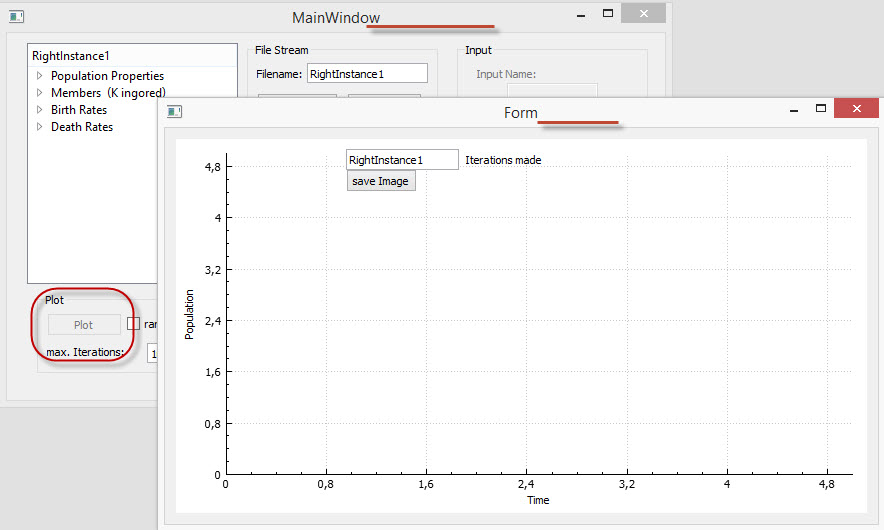
\includegraphics[width=1\linewidth]{./Pictures/PlotWindow_start}
		\caption[PlotWindow_start]{Start des PlotWindow}
		\label{PlotWindow_start}
	\end{figure}
	In blau sieht man, dass das Programm nicht eingefroren ist, als die Fenster "ubereinander gelegt wurden.\\
	Wenn die Simulation  einen g"unstigen Zustand erreicht hat oder die maximale Anzahl an gewünschten Iterationen absolviert hat, werden anschließend maximal 10mio Punkte auf dem Koordinatensystem zu Graphen verbunden (Abbildung \ref{PlotWindow_smallBPDL}). 
	\begin{figure}[H]
		\centering
		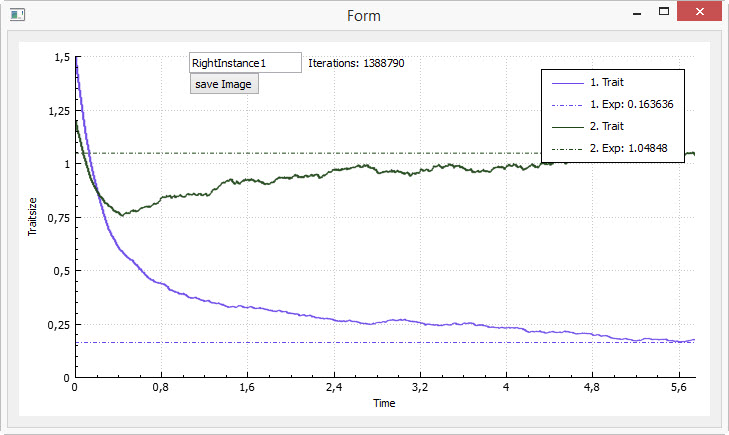
\includegraphics[width=1\linewidth]{./Pictures/PlotWindow_smallBPDL}
		\caption[PlotWindow]{PlotWindow mit Dimorpher Population}
		\label{PlotWindow_smallBPDL}
	\end{figure}
	
	Welche Optionen finden sich auf diesem Fenster?\\
	\begin{itemize}
		\item Nat"urlich kann man wie gew"unscht in einem Koordinatensystem die zeitliche Entwicklung der Population verfolgen.
		\item Dar"uber hinaus sieht man in gestrichelten Linien die stabilen Zust"ande der Population und kann die Konvergenz dahin verfolgen.
		\item Au"serdem ist bei aktiviertem "{}range Check"{} nicht klar, wie viele Iterationen (Spr"unge) tats"achlich gemacht wurden, um den aktuellen Zustand zu erreichen. Zu diesem Zweck ist mittig im Bild ein Label "{}Iterations: "{}, worin der Wert 1388790 zu sehen ist.
		\item In der rechten oberen Ecke findet sich au"serdem eine Legende der dargestellten Graphen. Dort sind im Wechsel die Merkmale mit ihrem erwarteten Gleichgewicht. "{}Exp"{} steht f"ur "{}Expected"{} und kennzeichnet den Gleichgewichtszustand.
		\item Des weiteren findet sich eine Schaltfl"ache "{}save Image"{} und eine Textbox, in die man den gew"unschten Bildnamen eintragen kann. Damit l"asst sich das Bild mit Legende als .pdf und .jpg abspeichern.
	\end{itemize}

	Was man zwar nicht direkt in Abbildung \ref{PlotWindow_smallBPDL} sehen kann, aber gut ausgearbeitet wurde, ist die Bewegungsfreiheit auf dem Bild.\\
	\begin{itemize}
		\item Mann kann in das Bild hineinzoomen.
		\item Die Messgitter werden beim zoomen automatisch angepasst.
		\item Auf dem Koordinatensystem kann man sich durch "{}Ziehen"{} bewegen.
		\item Das Fenster l"asst sich durch Strecken skalieren, wobei sich der Graph automatisch anpasst.
	\end{itemize}
	Als Beispiel dient Abbildung \ref{PlotWindow_zoomedBPDLmaximized}, welche durch Heranzoomen und Bewegen sowie maximierte Fenstergr"o"se (vgl. kleine Legende) erstellt wurde.
	\begin{figure}[H]
		\centering
		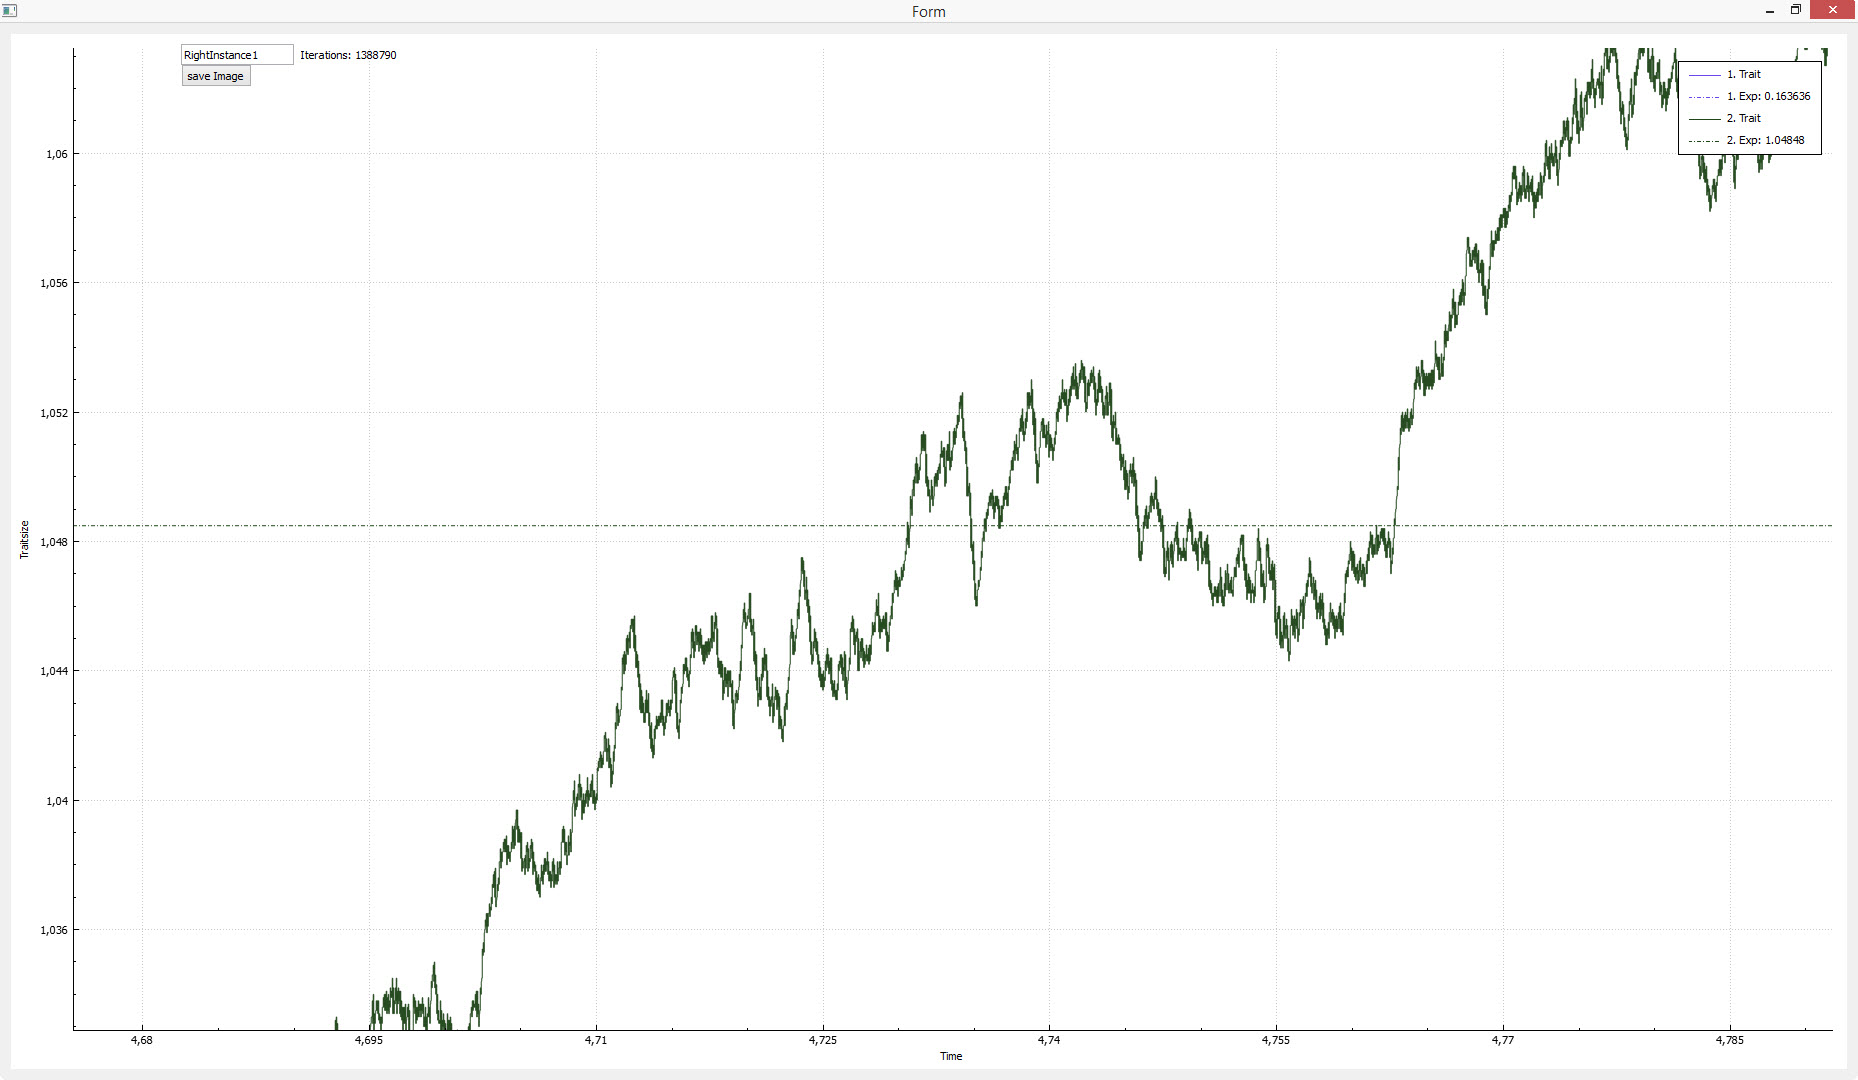
\includegraphics[width=1\linewidth]{./Pictures/PlotWindow_zoomedBPDLmaximized}
		\caption[PlotWindow]{PlotWindow mit Dimorpher Population}
		\label{PlotWindow_zoomedBPDLmaximized}
	\end{figure}
	Man kann sogar soweit skalieren, bis die Ereignisse lokal z"ahlbar werden und der Plot eine Gr"o"se hat in der das Messgitter eine Sprungmaschenweite hat:
	\begin{figure}[H]
		\centering
		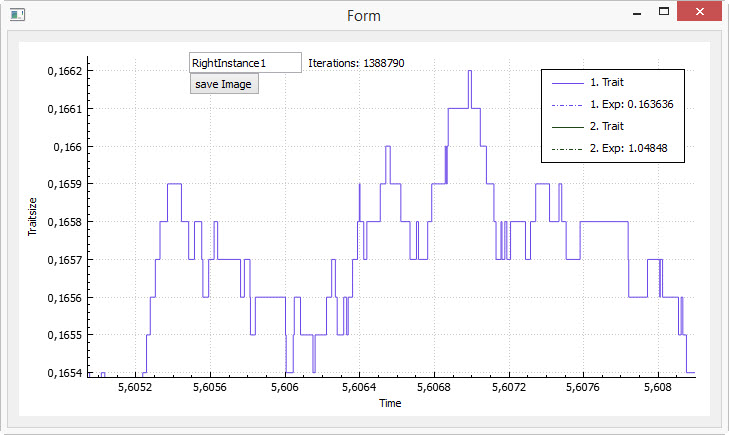
\includegraphics[width=1\linewidth]{./Pictures/PlotWindow_zoomedBPDL_Stepview}
		\caption[PlotWindow]{PlotWindow mit Dimorpher Population}
		\label{PlotWindow_zoomedBPDL_Stepview}
	\end{figure}	
	

\clearpage
\section{Verhaltenstests und Korrektheit der \\Implementation}
Ein ganz besonders interessantes Thema ist die Korrektheit der Implementation. Diese ist generell mit steigender Komplexität schwerer zu prüfen (besonders bei Zufallsbedingten Simulationen).\\
Daher habe ich mich dem Prinzip der "{}Testgetriebenen Entwicklung"{}  (Test Driven Develeopment - TDD) zugewendet \cite{martin2007professionalism}.\\
Wie der Name schon verr"at, geht es darum seine Entwicklung durch Tests, sogenannte "{}Unit Tests"{} anzutreiben. Diese Tests gew"ahrleisten kontrollierte Bedingungen um "Anderungen und Funktionalit"at so souverän wie m"oglich zu gestalten.\\
Das Konzept des TDD kann durch die Zusammenarbeit dreier Punkte aus \cite{martin2008clean} gut beschrieben werden:
\begin{itemize}
	\item[\textbf{1.}] Produktiver Code sollte nur geschrieben werden, um einen fehlgeschlagenen Unit Test bestehen zu lassen.
	\item[\textbf{2.}] Ein Unit Test sollte nur soweit entwickelt werden bis er fehlschl"agt.
	\item[\textbf{3.}] Es sollte nur so viel produktiver Code geschrieben werden, um einen Unit Test bestehen zu lassen. \label{3Punkte}
\end{itemize}

	\subsection{Unit Tests}
	Was ist ein Unit Test und was tut er?\\
	Ein Unit Test ist nichts anders als eine Funktion, die speziell daf"ur geschrieben wird, um ein implementiertes Verhalten bzgl. dem erwarteten Verhalten zu testen.\\
	Auf diese Weise w"urde nach den obigen 3 Punkten z.B. zun"achst eine Funktion (ein Test) geschrieben werden, die unser Modell mit Parametern initialisiert und z.B. pr"uft, ob die Geburtenrate f"ur diese Parameter gleich dem erwarteten Wert ist. Erst dann w"urde eine Geburtenraten-Funktion geschrieben werden, die den Test bestehen l"asst.\\ 
	Auf diese Weise l"asst sich oft eine deutlich effizientere Programmstruktur modellieren, als man es ursprünglich geplant hatte. Das Planen ist nat"urlich trotzdem ein wesentlicher Schritt. Mehr Einzelheiten zur Effizienz finden sich in \cite[The Bowling Game: An example of test-first pair programming]{martin2008clean}.\\
	In der Abbildung (\ref{Unit Test}) ist ein Beispiel für eine Implementation eines einfachen Tests, der prüft, ob alle Parameter korrekt aus der Datei in die Objekte geschrieben werden.\\
	Dazu werden in einer Schleife erst 1.000.000 mal immer wieder neu die Todesraten berechnet und pr"uft schlie"slich ob alle Raten trotzdem dem erwarteten Wert entsprechen (roter Kasten). Das ist Dank der modularen Implementierung, die in Kapitel 4 - Simulation vorgestellt wurde, m"oglich.
	\begin{figure}[H]
		\centering
		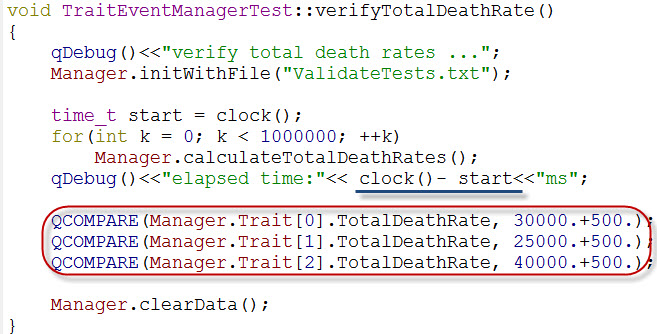
\includegraphics[width=1 \linewidth]{./Pictures/UnitTest_death}
		\caption[UnitTest]{UnitTest versichert korrekte Berechnung der Todesraten}
		\label{Unit Test}
	\end{figure}
	Startet man nun das Testprogramm, so werden der Reihe nach alle implementierten Tests gestartet. Die Ausgabe enth"alt Erfolge, Fehlschl"age und Zus"atzliche Debug-Ausgaben. Das ist in Abbildung \ref{Test Results} f"ur die ersten Tests des BPDL Programms vorgemacht worden. In rot sieht man den zuvor erw"ahnten Test:
	\begin{figure}[H]
		\centering
		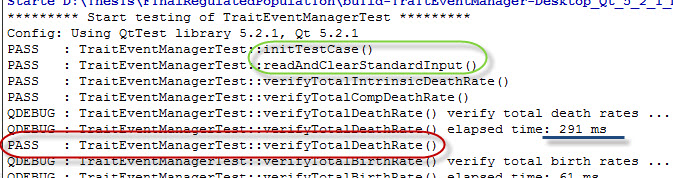
\includegraphics[width=1 \linewidth]{./Pictures/TestResult_start_death}
		\caption[Test Resultat einer Test Datei]{Ergebnisse einiger Tests}
		\label{Test Results}
	\end{figure}
	In blau sieht man dass auch der praktische Aufwand gemessen wurde um Schwachstellen in der Implementierung aufzudecken (z.B. auch beim Ziehen von Zufallsvariablen).\\
	
	\subsubsection{Korrektheit durch Unit Tests}
	Warum sollten ein paar Tests f"ur spezifische Situationen den Anspruch erheben Korrektheit des Programms zu gew"ahrleisten?\\
	Das Besondere an unserer Simulation ist, dass wir zuf"alliges Verhalten haben und deswegen oft nicht so einfach kleinere Fehler aufdecken k"onnen. Z.B. w"urde es in einer dimorphen BPDL Simulation nicht auffallen, wenn die Mutation unber"ucksichtigt bleibt solange die Wahrscheinlichkeit gering ist oder wenn die Zeiten zwischen Spr"ungen nicht richtig sind. Gerade deswegen wurde die "{}Testgetriebene Entwicklung"{} so interessant.\\
	Die Korrektheit eines Programmkerns nachzuweisen, kann sich als schwierig herausstellen, weil man die Korrektheit nicht f"ur eine spezifische Instanz, sondern flexibel f"ur alle nachweisen m"ochte.\\
	Doch ist es nicht notwendig die Flexibilit"at des Programms zu testen, wenn man stattdessen versucht, die Korrektheit jedes Arbeitsschrittes zu pr"ufen. Ein Arbeitsschritt erhebt in unserem Fall keinen Anspruch auf Komplexit"at. Tats"achlich sind unsere Arbeitsschritte alle m"oglichst einfach und erf"ullen nur eine Aufgabe. D.h. die Korrektheit der Arbeitsschritte zu verifizieren l"asst sich denkbar einfach mit einem Test abdecken.\\
	Wenn nun jeder Arbeitsschritt seine Aufgabe nachweisbar richtig erf"ullt, dann kann davon ausgegangen werden, dass durch richtige Verwendung der Arbeitsschritte das erwartete Verhalten eintritt.\\
	Die richtige Verwendung der Arbeitsschritte wird dadurch einfach nachzuweisen, dass wir im Kapitel 4 - "{}Simulation"{} den Algorithmus f"ur einen Evolutionsschritt vorgestellt haben. Dass dieser eine Schritt richtig ausgef"uhrt wird ist anhand des Pseudocodes leicht ersichtlich. Doch ist der n"achste Schritt nichts anderes als der erste Schritt, nur mit leicht ver"anderten Startwerten. Wenn also die Startwerte korrekt sind, dann wird auch der n"achste Schritt wieder richtig ausgef"uhrt.\\
	Auf diese Weise wird die Komplexit"at der Simulation vereinfacht auf die der Ablaufpunkte, die im wesentlichen sehr einfach sind.\\
	Was allerdings nicht gepr"uft wurde, ist der Umgang mit den erhobenen Daten innerhalb des "{}GUI"{} Moduls. Leider ist mir nicht bekannt, wie sich Tests auf ereignisgesteuerten Code entwickeln lassen, womit nur zwei von den drei in Abbildung (\ref{Module und Klassen}) beschriebenen Modulen getestet werden konnten.

	\subsection{Unit Tests des Programmkerns}
	Hier werden Tests vorgestellt mit denen die korrekte Berechnung der Raten verifiziert werden soll. Dazu wird die folgende Testinstanz mit 3 Merkmalen ($ X = \{x,y,z\} $) verwendet:\\
	\begin{center}
		\begin{minipage}{0.35 \textwidth}
			\begin{tabular}{ c | c c c }
			 $ c(\cdot, \cdot) $ & x & y & z \\
			 \hline
			 x & 2 & 1 & 0 \\
			 y & 0 & 2 & 0.5 \\
			 z & 0 & 2 & 2 \\
			\end{tabular}
			\end{minipage}
			\begin{minipage}{0.5 \textwidth}
			\begin{tabular}{ c | c  c  c  c  c  c  c }
			 & $ b(\cdot ) $ &  & $ d(\cdot ) $ & & $ n(\cdot ) $ & & $ \mu $\\
			 \hline
			 x & 10 &  & 5 & & 100 & & 0.1\\
			 y & 10 &  & 5 & & 100 & & 0.1\\   
			 z & 10 &  & 5 & & 100 & & 0.1\\
			\end{tabular}
			\end{minipage}
	\end{center}
	Es wurden 3 Merkmale gew"ahlt, weil es die minimale Anzahl ist, um die Auswirkungen von "{}inneren"{} Merkmalen auf Rand-Merkmale (und umgekehrt) zu testen.\\
	Vor den Kerntests wurden noch Tests gemacht, die versichern, dass kein Fehler beim Lesen, Schreiben, Neulesen, Ver"andern etc. der Raten und Parameter auftritt. Diese sind z.B. in gr"un in Abbildung \ref{Test Results} zu sehen.

	\subsubsection{Raten}
	Das Testen der Todesraten l"auft auf den finalen Todesraten Test aus Abbildung (\ref{Unit Test}) hinaus. Diese zeigt die Implementation des entsprechenden Tests. Jede weitere Implementation kann im Quellcode nachgesehen werden, jedoch werden hier nur heuristisch die Tests aufgelistet um die Qualit"atstests nachvollziehbar zu machen. In den Tests selber wird stets jedes Merkmal und dessen Werte auf Korrektheit gepr"uft, obwohl folgend immer nur ein Merkmal vorgerechnet wird.\\
	
	\textbf{Intrinsische Todesrate:}\\
	Exemplarisch an $ y $ erwarten wir f"ur diese Instanz folgende Berechnung,\\
	\renewcommand{\arraystretch}{1.2}
	\begin{tabular}{c l}
		\underline{Erwartet}: 		& $ d(y) \cdot n(y)  $\\
						& $ = 5 \cdot 100 = 500 $ \\\\
		\underline{Testergebnis}: 	& $ \trvec{500}{500}{500} $
	\end{tabular}\\\\
	Der Vergleich mit dem Testergebnis best"atigt somit das Verhalten der intrinsischen Todesraten Berechnung.\\
	
	\textbf{Todesrate durch Wettbewerb:}\\
	Erneut an $ y $ erwarten wir f"ur diese Instanz folgende Berechnung,\\
	
	\begin{tabular}{c l}
		\underline{Erwartet}: 		& $ n_0(y) \cdot \sum_{w \in X} c(y,w) \cdot n_0(w) $\\
						& $ = 100 \cdot ( 2 \cdot 100 + 0.5 \cdot 100 ) = 25000 $\\\\
		\underline{Testergebnis}: 	& $ \trvec{30000}{25000}{40000} $
	\end{tabular}\\\\
	Wie erwartet best"atigt sich das Ergebnis f"ur $ y $. Durch den gro"sen Abstand zum Equilibrium beider Funktionen entsteht hier nat"urlich eine gro"se wettbewerbliche Todesrate. Au"serdem l"asst sich beobachten, dass f"ur das letzte Merkmal $ z $ die gr"o"ste Rate berechnet wurde, was einfach an der Zeilensumme der Wettbewerbsmatrix begr"undet werden kann.\\
	
	\textbf{Totale Todesraten:}\\
	Hier muss nicht mehr viel vorbereitet werden. Wir haben bereits die intrinsische und wettbewerbliche Todesrate ausgerechnet. \\
	
	\begin{tabular}{c l}
		\underline{Erwartet}: 		& $ D(y) =  d(y) \cdot n(y) + n_0(y) \cdot \sum_{w \in X} c(y,w) \cdot n_0(w) $\\
						& $ = 500 + 25000 = 25500$\\\\
		\underline{Testergebnis}: 	& $ \trvec{30500}{25500}{40500} $
	\end{tabular}\\\\
	Wie erwartet best"atigt sich das Ergebnis f"ur $ y $. In Abbildung \ref{Test Results} kann man die Ausf"uhrung aller 3 Tests noch verfolgen.\\
	In anderen Tests (des TSS Programms) wurden die selben Tests noch f"ur unterschiedliche Instanzen gemacht. Das erm"oglicht es davon auszugehen dass die Todesraten korrekt berechnet werden.\\
	
	\textbf{Totale Geburtenraten:}\\
	Hier wird exemplarisch erneut das mittlere Merkmal $ y $ verwendet, welches durch die Mutation von beiden Seiten eine h"ohere Geburtenrate erwartet. \\
	
	\begin{tabular}{c l}
		\underline{Erwartet}: 		& $ B(y) = (1-\mu) \cdot b(y) \cdot n_0(y) + \frac{\mu}{2} \cdot \left( \sum_{w \in X} b(w) \cdot n_0(w) \right) $\\
						& $ = 10 \cdot 100 + 0.05 \cdot (10 \cdot 100 + 10 \cdot 100) = 1000$\\\\
		\underline{Testergebnis}: 	& $ \trvec{950}{1000}{950} $
	\end{tabular}\\\\
	Die Geburtenraten unterscheiden sich nur zwischen Rand und Innerem um  $ 50 $, da wir die mutative Geburtenrate $ 0.05 \cdot 10 \cdot 100 = 50 $ von Links und Rechts an Randmerkmalen nat"urlich nur einmal erhalten.\\
	
	\textbf{Totale Raten:}\\
	Dank der vorherigen Schritte l"asst sich die Totale Merkmalsrate leicht berechnen.\\
	
	\begin{tabular}{c l}
		\underline{Erwartet}: 		& $ B(y) + D(y) = $\\
						& $ 1000 + 25500 $, bzw. $ \trvec{950}{1000}{950} + \trvec{30500}{25500}{40500} = \trvec{31450}{26500}{41450} $\\\\
		\underline{Testergebnis}: 	& $ \trvec{31450}{26500}{41450} $
	\end{tabular}\\\\
	Schlie"slich folgt daraus auch die Totale Ereignisrate.\\
	
	\begin{tabular}{c l}
		\underline{Erwartet}: 		& $ 31450 + 26500 + 41450 = 99400 $\\\\
		\underline{Testergebnis}: 	& $ 99400 $
	\end{tabular}\\\\
	Das beendet die wesentlichen Tests zur Berechnung der Raten.
	
	\subsubsection{Ziehen einer Ereigniszeit}
	In diesem zweiten Teil der Tests werden Ereigniszeiten gezogen und mit dem Gesetz der gro"sen Zahlen der Mittelwert mit dem erwarteten Mittelwert verglichen.\\
	Es gab noch weitere Tests, die hier nicht erw"ahnt werden, weil sie blo"s testen, ob der verwendete "{}W"urfel"{} wirklich unabh"angige Ziehungen macht und ob die Verteilung das tut, was sie soll.\\
	
	\textbf{Geburts- und Todeszeitpunkte:}\\
	Um diese Ziehung zu verifizieren wurden $ 1.000.000 $ Ereigniszeitpunkte mit den selben Raten gezogen und gemittelt.\\
	Der Erwartungswert dieser Ziehung entspricht $ \frac{1}{\text{TotalEventRate}} $ was auch der Referenzwert f"ur die Fehlerberechnung ist. F"ur das Testergebnis wird eine absolute Genauigkeit von $ 99.995 \% $ gefordert und der Fehler erreicht meistens einen Wert um $ 0.0008\% $ herum.\\
	
	\textbf{TSS Mutationszeiten:}\\
	F"ur die korrekte Ziehung der Mutationszeitpunkte in einer TSS Simulation wird eine etwas andere Testinstanz verwendet, die nicht entscheidend ist, aber in allen TSS Testinstanzen verwendet wird. Diese Instanz ist unter dem Namen "{}ValidateTSSTests.txt"{} im Programmordner zu finden und stellt sicher, dass die Fitness einen Wechsel der Merkmale garantiert.\\
	Um die Mutationszeiten zu validieren wird 100.000 mal der folgende Ablauf durchgegangen:
	\begin{itemize}
		\item[\textbf{1}] Zun"achst werden alle bis auf ein Merkmal get"otet.
		\item[\textbf{2}] Das "ubrige Merkmal wird auf sein Gleichgewicht gehoben.
		\item[\textbf{3}] Dann wird eine Funktion aufgerufen, die sp"ater im n"achsten Kapitel vorgestellt wird und den Zeitpunkt der n"achsten Mutation aus den Mutationsraten zieht.
		\item[\textbf{4}] Dieser Zeitpunkt wird zu vorhergehenden Zeiten summiert.
	\end{itemize}
	Nach der Schleife wird nat"urlich das Mittel gezogen und auf eine absolute Genauigkeit von $ 99.95\% $ gepr"uft. Die Testergebnisse lagen in der Regel bei einem Fehler um $ 0.002\% $ herum.\\
	
	\subsubsection{Ver"anderung der Population}
	Wie vielleicht bemerkt wurde, kommen wir zum letzten Bereich der Aufteilung aus Abbildung \ref{fig:PseudoCodeForBThesis} Level 1.\\
	
	\textbf{Merkmal ausw"ahlen}\\
	Um zu verifizieren, dass die Merkmale korrekt den Ereignissen zugeteilt werden, wurde ein Histogramm der Wahlen erstellt. Genau gesagt wurde 100.000 mal entschieden, welches Merkmal ein Ereignis ausl"osen wird.\\
	Wie schon in Kapitel 4 - "{}Simulation"{} erw"ahnt, ist es sehr n"utzlich gewesen die Raten getrennt zu berechnen und zu speichern. Von diesem Vorteil kann jetzt Gebrauch gemacht werden um zu unterscheiden welches Merkmal wie viele der 100.000 Ereignisse ausgel"ost h"atte.\\
	Die getestete Genauigkeit war $ 99.95\% $ und wie zuvor haben die Ergebnisse sie stets ausreichend "uberschritten.\\
	
	\textbf{Ereignis Typ w"ahlen}\\
	Die Idee dieses Tests ist praktisch identisch zum Vorherigen und wird nicht n"aher beschrieben, ist aber nat"urlich ausf"uhrlich im Quellcode vorhanden und hat ebenso bestanden.\\
	
	\textbf{Ereignis ausf"uhren}\\
	Hier wurde nur schnell getestet, ob das Ausf"uhren eines gew"ahlten Ereignisses auf ein gew"ahltes Merkmal korrekt abl"auft. Dabei wurde lediglich gepr"uft, ob bei einer Geburt wirklich die Population anw"achst und bei Tod bis zu einem Minimum von 0 sinken kann.
	
	\subsection{Unit Tests der Konvergenz}
	Hier wurde erstmal gepr"uft, ob das vom Programm ermittelte Gleichgewicht wirklich richtig berechnet wurde.\\
	Schlie"slich wurde noch f"ur dimorphe und monomorphe Populationen getestet, ob und wie gut die Konvergenz f"ur wachsende K zum Gleichgewicht abl"auft. Hierzu wurden 1.000.000 Spr"unge des Prozesses mit $ K = 10 $ und $ K = 10.000 $ gemacht. F"ur $ K = 10 $ bewegt sich der Fehler um $ 0.1\% $ und f"ur $ K = 10.000 $ um $ 0.001\% $. Besonders bei gro"sem $ K $ konnte man beobachten, dass der Fehler der dimorphen Population oft korreliert d.h. oft waren beide gering oder hoch.
	
	
\clearpage
\section{TSS Prozesse}
In diesem Kapitel geht es um TSS Prozesse und wie eine Ann"aherung dieser durch unsere Simulation gel"ost wurde.
	\subsection{Invasion}
	Wie schon in Kapitel 3.4 der Fitnessfunktion angesprochen, beschreibt die Invasion den Vorgang, durch den ein neu auftretendes Merkmal (dank Mutation) ein bis dahin dominantes Merkmal verdr"angt.\\
	In Kapitel 3.2 haben wir weiterhin gesehen, dass der BPDL-Prozess f"ur $ K \to \infty $ gegen ein deterministisches System konvergiert. Jedoch soll unser TSS-Prozess ein nicht deterministischer Prozess sein, der eine monomorphe Population simuliert, die zu zuf"alligen Zeiten ihr dominantes Merkmal austauscht.\\
	Um dies zu erreichen wird der Grenzwert nicht nur mit $ K \to \infty $, sondern gleichzeitig $ \mu \to 0 $ gebildet. Auf diese Weise wird das sonst so deterministische Verhalten aus $ K \to \infty $ durch weiterhin zuf"allige Ereignisse beeinflusst.\\
	Dabei wird der aus Kapitel 3.6 bekannte Bereich (\ref{TSSMutation}) f"ur die Konvergenz von $ \mu $ gew"ahlt. Er garantiert, dass eine Invasion ausreichend Zeit zur Verdr"angung hat bis ein weiterer Mutant entsteht und nicht zu viel Zeit vergeht, so dass das vor der n"achsten Mutation die Population ausstirbt.\\
	Desweiteren wollen wir auch sicherstellen, dass sich auf lange Sicht nur ein Merkmal durchsetzt. Dies k"onnen wir erreichen, indem wir ausnutzten, dass stets zwei Merkmale um Dominanz streiten und die Aussagen aus Kapitel 3.5 (Dimorphes Gleichgewicht) auf mehrere Merkmale ausweiten.\\
	Wenn f"ur beliebiges $ x \in X $ und f"ur alle $ y \in (X\backslash x) $ entweder $ f(y,x) < 0 $ oder $ f(y,x) > 0 $ und $ f(x,y) < 0 $, so ist sichergestellt, dass sich auf lange Sicht ein Merkmal in der Population durchsetzten wird und keine zwei Merkmale nebeneinander existieren k"onnen. Unter diesen Umst"anden k"onnen weiterhin die stabilen monomorphen Zust"ande die in Kapitel 3.5 (Dimorphes Gleichgewicht) beschrieben wurden angenommen werden, nur eben f"ur mehrere Merkmale.\\
	
	\textbf{Welche Phasen durchl"auft eine Invasion?}\\
	Damit ein Merkmal y ein dominantes Merkmal x verdr"angen kann, muss nach obigen Erkenntnissen zun"achst einmal $ f(y,x) > 0 $ und $ f(x,y) < 0 $ gelten.\\
	Wie aus \cite{Silke}, l"asst sich die Invasion in 3 Teilen beschreiben. 
	\begin{itemize}
		\item [1.] Fixierung: Zu Beginn einer Invasion werden die Individuen des Merkmals $ x $ kaum von $ y $ beeinflusst, da $ c(x,y)n(y) $ unbedeutend klein ist. Jedoch ist dieser Zustand zeitlich durch die positive Wachstumsrate des Merkmals $ y $ f"ur $ x $ im Gleichgewicht $ \bar{n}_x $ begrenzt. Ab einer bestimmten Populationsgr"o"se $ \eps $, kann der Einfluss des Eindringlings $ x $ von $ y $ nicht mehr ignoriert werden. Die Dauer bis ein erster Mutant das Merkmal zu diesem relevanten Niveau bringt, hat die Gr"o"senordnung $ \log K $.
		\item [2.] Invasion: Hier ereignet sich der rasche Abfall des dominanten Merkmals $ x $ und Anstieg des neuen Merkmals $ y $. Wir beobachten hier die Konvergenz gegen den, dank $ f(x,y) < 0 $ und $ f(y,x) > 0 $, Gleichgewichtszustand $ (0,\bar{n}_y) $.
		\item [3.] Aussterben: Hier greift der Umgekehrte Fall der Fixierung. Sobald $ n(x) < \eps $ geworden ist, kann zun"achst der Einfluss von $ x $ auf $ y $ vernachl"assigt werden und dank der negativen Wachstumsrate wird das Merkmal $ x $ in einer Zeit von der Ordnung $ \log K $ aussterben.
	\end{itemize}
	Beispielhaft kann man das an folgenden Abbildungen beobachten:\\
	\begin{minipage}{0.7 \textwidth}
	\begin{figure}[H]
		\centering
		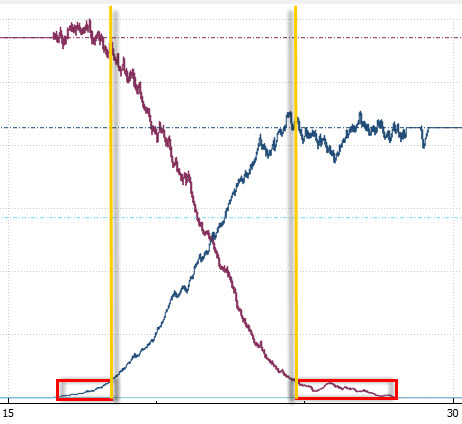
\includegraphics[width=1 \linewidth]{./Pictures/Invasion2}
		\caption[Invasion]{Eine Invasion f"ur K = 1000}
		\label{Invasionsphasen}
	\end{figure}
	\end{minipage}
	\begin{minipage}{0.3 \textwidth}
		In rot sind die Fixierungsphasen gekennzeichnet und in orange erkennt man die Zeitpunkte, an denen die "Uberg"ange beobachtbar sind.
	\end{minipage}\\
	
	\textcolor{blue}{Man kann in dieser Stelle bereits erahnen, dass die Fitnessfunktion bzw. die Wachstumsrate eines Mutanten die M"oglichkeit bietet, Aussagen "uber die Invasionswahrscheinlichkeit zu machen. Und tats"achlich erhalten wir aus \cite{Champagnat20061127}, dass die Invasionswahrscheinlichkeit mit $ K \to \infty $ gegen
	\[ \frac{\left[ f(y,x)\right]_+ }{b(y)} \]
	konvergiert.} 
	
	\subsubsection{Praktische Umsetzung}
	Normalerweise lassen sich die Parameter einer Simulation so w"ahlen, dass bei mindestens drei Merkmalen ein Kreislauf der Invasionen erzwungen werden kann. D.h. es wird nicht dazu kommen, dass ein Merkmal nicht verdr"angt werden kann, also: $ x \xleftarrow{verdr"angt} y \xleftarrow{verdr"angt} z \xleftarrow{verdr"angt} x \dots $\\
	In unserem Modell jedoch haben wir nur Mutationen zu den Nachbarn erlaubt. Diese Einschr"ankung verhindert den Kreislauf. Wenn ein Merkmal $ y $ ein $ x $ verdr"angt, so kann es nicht mehr von selbigem $ x $ verdr"angt werden, sondern muss vom anderen Nachbarn verdr"angt werden.\\
	Auf diese Weise wandert die Vorherrschaft in der Population bis ein Merkmal dominant ist, welches keine fitteren Nachbarn hat oder am Rand angekommen ist, was zwangsl"aufig wieder dem vorherigen Fall entspricht.\\
	Die Darstellung der Fitnessmatrix im Programm l"asst sich an folgendem Bild leicht nachvollziehen:
	\begin{figure}[H]
		\centering
		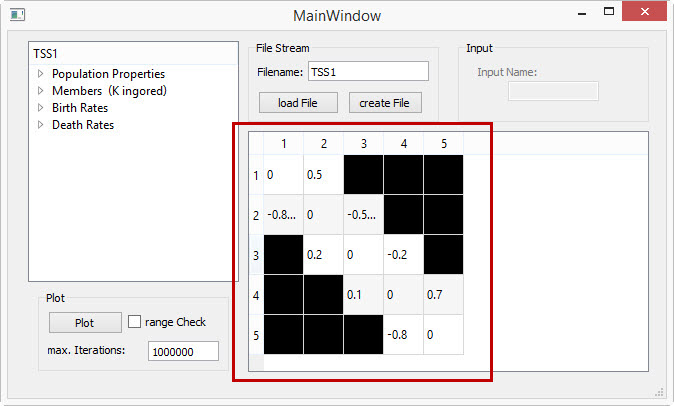
\includegraphics[width=1\linewidth]{./Pictures/MainWindow_BandMatrix}
		\caption[Fitness Matrix]{Fitness Bandmatrix}
		\label{MainWindow mit Fitness Bandmatrix}
	\end{figure}
	Da die Fitness nicht die einzige n"utzliche Information bei Invasionen ist, wurde dem Programm noch die M"oglichkeit gegeben farblich darauf hinzuweisen, ob ein Invasion m"oglich ist und ob sie besonders wahrscheinlich ist.\\
	Dazu folgendes Bild:
	\begin{figure}[H]
		\centering
		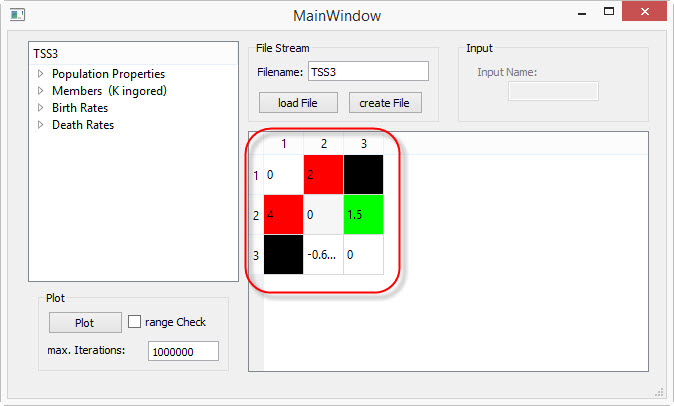
\includegraphics[width=1\linewidth]{./Pictures/MainWindow_red_green_loaded}
		\caption[MainWindow_redGreenFitness]{Fitness Matrix mit roten und gr"unen Akzenten}
		\label{fig:MainWindow_red_green_loaded}
	\end{figure}
	Dabei werden drei Farben unterschieden. 
	\begin{itemize}
		\item [\textbf{Rot}] werden beide Merkmale gef"arbt, falls wir einen Zustand der Koexistenz erwarten. In diesem Fall sind $ f(x,y) \& f(y,x) > 0 $.
		\item [\textbf{Wei"s}] wird ein Merkmal gef"arbt, wenn es verdr"angen oder verdr"angt werden kann.
		\item [\textbf{Gr"un}] wird ein Merkmal gef"arbt, wenn die Verdrängungswahrscheinlichkeit "uber 60\% ist.
	\end{itemize}

	\subsection{Optimierung}
	Einfach den BPDL-Simulator zu verwenden, um diesen Grenzwertprozess zu approximieren, w"urde darin resultieren, dass sehr viel Rechenzeit im Gleichgewicht eines Merkmals verbracht werden w"urde.\\
	Die Beobachtung des Prozesses im Gleichgewicht ist nicht besonders interessant und es l"asst sich dabei nicht gut nachvollziehen, wann vielleicht Mutanten Invasionsversuche gestartet haben, die nicht durchgekommen sind. Diese Simulation wurde bereits in Abbildung (\ref{TSS_mitBPDLSimulator}) vorgestellt.\\
	Alternativ wird hier eine andere Variante dieser Simulation vorgestellt. 
	Diese nutzt eine lineare Interpolation als eine Optimierung um die "Ubersichtlichkeit, Analysef"ahigkeit und Laufzeit deutlich zu verbessern.\\
	Diese lineare Interpolation macht es notwendig, stets zu wissen in welcher der drei Phasen der Prozess sich zur Zeit bewegt. Sobald er die Aussterben Phase verlassen hat und schlie"slich der Prozess sein Equilibrium erreicht, wird eine Interpolation des Prozesses bis zu seiner n"achsten Mutation durchgef"uhrt.\\
	Die Spr"unge bis zum n"achsten Mutanten werden nicht berechnet, stattdessen wird anhand der Geburtenrate der toten Nachbarn eine Mutationsrate zusammengefasst, welche uns die Zeit f"ur die n"achste Mutation liefert. Danach wird nach dem selben Vorgehen, wie in Kapitel 4 beschrieben, entschieden, welcher Nachbar die Mutation ausgel"ost hat.\\
	\begin{figure}[H]
		\centering
		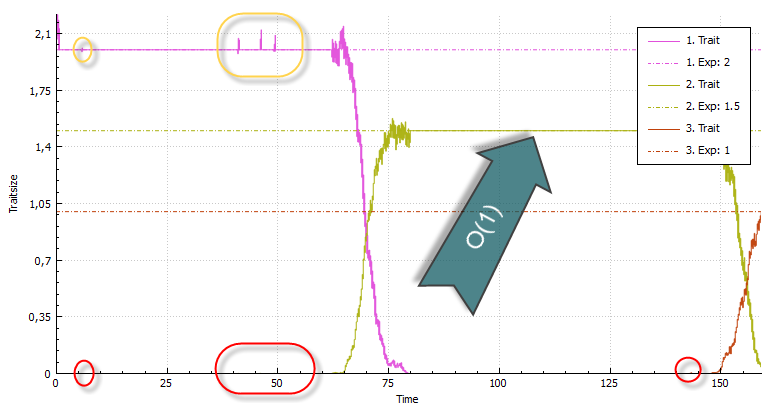
\includegraphics[width=1\linewidth]{./Pictures/TSS2_optimierung_small}
		\caption[MainWindow_redGreenFitness]{optimierte Simulation einer TSS Approximation}
		\label{TSS2_optimierung_small}
	\end{figure}
	Das sich dadurch die gr"o"ste Rechenzeit auf $ O(1) $ verk"urzt und die "Ubersichtlichkeit verbessert ist sehr deutlich und war zu erwarten. Die Analysem"oglichkeiten jedoch verbessern sich dank des gro"sen Ratenunterschiedes der Merkmale. Der eindringende Mutant bietet dem neuen Merkmal nur eine sehr geringe Ereignisrate. W"ahrend dieser Zeit sind gro"se Bewegungen im dominanten Merkmal zu erwarten. Diese Beobachtung l"asst sich leicht in Abbildung (\ref{TSS2_optimierung_small}) nachvollziehen, wo man in rot niemals einen Mutanten entdecken w"urde, jedoch dank der Ausschl"age in der gelben Markierung ist es einfach die Mutanten aufzusp"uren.\\
	Folgend werden beide Effekte gegen"ubergestellt:\\
	\begin{center}
	\begin{minipage}{0.6\textwidth}
	\begin{minipage}{0.45\textwidth}
		\centering
		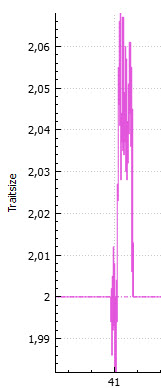
\includegraphics[width=1\linewidth]{./Pictures/TSS_DomZoomVgl_original}
		\label{a}
	\end{minipage}
	$ \quad $
	\begin{minipage}{0.45\textwidth}
		\centering
		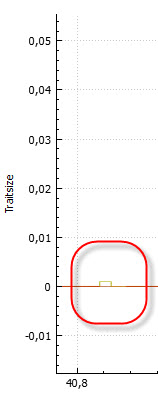
\includegraphics[width=1\linewidth]{./Pictures/TSS_MutationZoomVgl2_original}
		\label{b}
	\end{minipage}
	\end{minipage}
	\end{center}	
	Nat"urlich ist es dank der Beweglichkeit auf dem Graphen auch m"oglich, die Entwicklung des Mutanten n"aher zu betrachten:
	\begin{figure}[H]
		\centering
		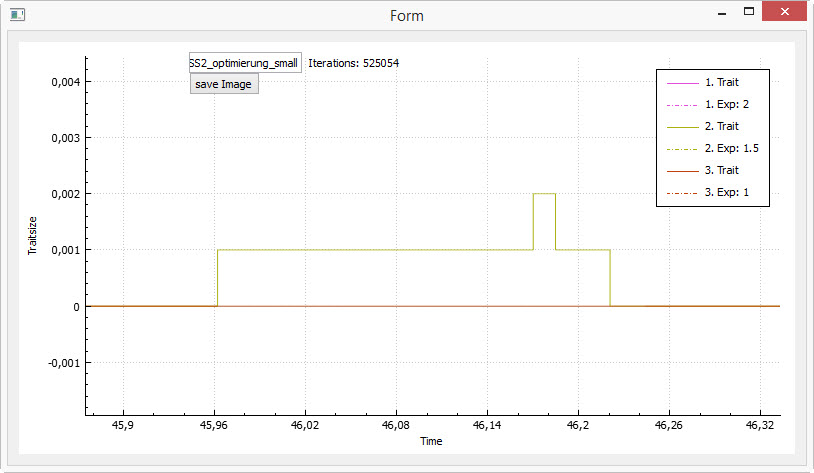
\includegraphics[width=1\linewidth]{./Pictures/TSS_MutationZoom2_original}
		\caption{Dritte Mutation von Links}
		\label{TSS_MutationZoom2_original}
	\end{figure}
	
	\subsection{Implementierung}
	Welche Form die Implementierung und der Algorithmus annehmen, wurde bereits in Kapitel 4 ausreichend erl"autert. Deswegen wird hier nur kurz erkl"art wie sich der Algorithmus "andern w"urde. Die tats"achliche Implementierung weicht etwas ab und verwendet technisch unwichtige Details.\\
	
	\textbf{Implementierung}
	Die Implementierung ben"otigt jetzt, bevor es einen gew"ohnlichen Sprung macht, zus"atzlich eine "Uberpr"ufung ob wirklich ein Prozesssprung oder eine Mutation ausgef"uhrt werden soll.\\
	Dazu wird nach jedem Sprung eine Abfrage "isNear()" gestartet, die pr"uft ob es nur ein lebendes Merkmal gibt und ob es im Gleichgewicht ist:
	\begin{algorithm}[H]
		\caption{isNear()}
		\begin{algorithmic}[1]
			\Ensure{Bedingungen f"ur eine Interpolation}
			\For{ i = 0 < n-1}
				\If{i $ \ne $ ChosenTrait \& Members[i] $ > 0$}
					\Return false;
				\EndIf
			\EndFor
			\If{$ |\text{getKMembersOf[i]} - \text{Expected[ChosenTrait]}| > \frac{0.5}{K} $}
				\Return false;
			\EndIf
			\Return true;
		\end{algorithmic}
	\end{algorithm}
	Hier sorgt Zeile 2 in der Schleife daf"ur, dass au"ser dem zuletzt aktiven kein weiteres Merkmal aktiv sein k"onnte.\\
	Danach wird in Zeile 6 sicher gestellt, dass der Abstand zum Gleichgewicht minimal ist. Das ist notwendig, denn der Minimale Abstand ist nicht immer $ 0 $. Falls das Gleichgewicht einen Wert ergibt, der kein Vielfaches von $ \frac{1}{K} $ ist, so kann das Gleichgewicht nicht durch den Prozess angenommen werden. In diesem Fall wird der Prozess jedoch stattdessen einen Sprungpunkt im Radius $ \frac{0.5}{K} $ um das Gleichgewicht haben.\\
	Als Abbruchkriterium wird nicht mehr einfach die maximale Anzahl erlaubter Spr"unge verwendet, sondern auch ein Interpolationspunkt des Merkmals, an dem keine fitteren Nachbarn mehr vorhanden sind. Die Implementierung des Abbruchkriteriums sollte intuitiv sein und wird deshalb nicht weiter beschrieben.\\
	
	\textbf{Aufwand}\\
	Eine Besonderheit l"asst sich zum Schluss noch betonen. Durch die Interpolation ist der Aufwand der Berechnung nicht mehr allein von K abh"angig, sondern besonders von der Anzahl der erwarteten Mutationen und der Anzahl der erwarteten Invasionen.
	

\clearpage
\section{Ausblick}
Schon fr"uh war klar, dass noch viele M"oglichkeiten offen bleiben werden, wie die Simulation erweitert werden kann. Einige gr"o"sere Anpassungen, von denen noch einige nach dem Erstellen dieser Arbeit implementiert werden, werden hier kurz vorgestellt:
\begin{itemize}
	\item[1.] Dank der hier verwendeten Art der Implementierung ist das Erweitern des Programmkerns auf alternative Modelle denkbar einfach. So w"are es sehr einfach die Mutationswahrscheinlichkeit nicht nur mit gleichen Teilen auf die Nachbarn mit zu verteilen, sondern eine individuelle Wahrscheinlichkeit auf beliebige Merkmale. Dazu muss nur die Einlesefunktion der Parameter und die Berechnung der mutativen Geburtenrate ver"andert werden. Alle anderen Teile des Programms w"aren davon unbeeinflusst. Insbesondere garantieren die bereits geschriebenen Tests dass bei einer Ver"anderung am Programmkern keine unbemerkten negativen Effekte auftreten. Nat"urlich w"are damit das Abbruchkriterium der TSS Simulation hinf"allig, aber es w"urden keine Fehler verursachen.
	\item[2.] Weiterhin kann die Darstellung des Graphen im TSS Simulator optimiert werden. So kann z.B. die Zeit zwischen den Mutationen gestaucht werden, so dass es einfach wird nur die "Uberg"ange und Mutationen genauer zu betrachten. \\
	Au"serdem k"onnte es eine M"oglichkeit geben die Bilder des Programms als Vektorgraphiken abzuspeichern oder an einer Stelle des Prozesses mit ge"anderten Parameter weiter simulieren.
	\item[3.] Man k"onnte einen Popupcontainer implementieren, der zus"atzliche Anzeigedaten f"ur den Plot erm"oglicht. Z.B. k"onnte man so die Legende mit weiteren Parameter, wie $ \mu_K, K $ oder anderen f"ullen. Au"serdem k"onnte es eine Option enthalten, die Anzahl der relevanten Invasionsversuche eines Merkmals anzuzeigen.\\
\end{itemize}
In einem Protokoll, das neben der Entwicklung des Programms geschrieben wurde, werden stichpunktartig "uber zwei Seiten gro"se und kleine Erweiterungen sowie Verbesserungen aufgez"ahlt. Die Implementierung des Programms erm"oglicht eine flexible Weiterentwicklung, weshalb sich schnell viele Punkte sammeln.


\clearpage
\bibliography{science1}





\end{document}